
%%---------------------------------------------------------------------------------------------------------------------- Preamble

\documentclass[11pt]{report}

\newcommand{\code}[1]{\texttt{#1}}
\usepackage[a4paper,left=3cm,right=3cm,bottom =2cm]{geometry}

%\usepackage{natbib}

% urls in sources
\usepackage{url}
\usepackage{graphicx}

% chapter headers format
\usepackage{titlesec}
\titleformat{\chapter}
  {\normalfont\bfseries\Huge}{\thechapter}{22pt}{\Huge}

\makeatletter
\let\my@chapter\@chapter
\renewcommand*{\@chapter}{%
  \addtocontents{lol}{\protect\addvspace{10pt}}%
  \my@chapter}
\makeatother

% acronyms
\usepackage{array}
\usepackage{acro}
\acsetup{list/template=tabular}
\DeclareAcronym{gui}{
  short = GUI,
  long = graphical user interface,
  list = Graphical User Interface
}

% line spacing
\usepackage{setspace}

% links in references
\usepackage[hidelinks]{hyperref}

% smart references
\usepackage[noabbrev,nameinlink]{cleveref}

% wrap text around images
\usepackage{wrapfig}

% line spacing
\usepackage{setspace}
\setstretch{1.25}

% float at exactly here
\usepackage{float}

% rotate figures
\usepackage{adjustbox}
\usepackage{blindtext}

%for multiline tables
\usepackage{multirow}
\usepackage{tabularx}

%thick lines
\usepackage{booktabs}

%bibliography/ references
\usepackage[backend=bibtex]{biblatex}

%%Wallpaper package
\usepackage{wallpaper,lipsum}

%%Textpos package
\usepackage{textpos}

\usepackage{listings}
\usepackage{color}

%Wrapping Picture around text
\usepackage{wrapfig}

%Code highlighting
\usepackage[outputdir=D:/AIN_Ubiquitous_Computing/doc/outdata]{minted}
\usemintedstyle{perldoc}
\usepackage{xcolor} % to access the named color LightGray


%forest
\usepackage{forest}

\def\Size{4pt}
\tikzset{
  folder/.pic={
    \filldraw[draw=folderborder,top color=folderbg!50,bottom color=folderbg]
      (-1.05*\Size,0.2\Size+5pt) rectangle ++(.75*\Size,-0.2\Size-5pt);  
    \filldraw[draw=folderborder,top color=folderbg!50,bottom color=folderbg]
      (-1.15*\Size,-\Size) rectangle (1.15*\Size,\Size);
  }
}

\usepackage{graphicx}
\usepackage{caption}
\usepackage{subcaption}


% list all used packages and their versions to the logfile
\listfiles

%%---------------------------------------------------------------------------------------------------------------------- Defines

%% Project defines.
%------------------------------------------------------------------------------- PATH
\newcommand{\projectPath}{/mnt/c/Projects/AIN_Ubiquitous_Computing/doc}      % Path to the project.
\newcommand{\sectionsPath}{\projectPath/sections}	                            % Sections path
\newcommand{\outdataPath}{\projectPath/outdata}                                 % Output path
\newcommand{\outdir}{outputdir=\outdataPath}

%Document Title
\newcommand{\docTitle}{Ubiquitous Computing WS 24}
\newcommand{\docSubTitle}{Exercises Documentation}

%Creator information
\newcommand{\docCreater}{}
\newcommand{\docCreaterID}{}
\newcommand{\docCreatorMail}{}

%Location and date
\newcommand{\docLocation}{}
\newcommand{\docDate}{}

%Background picture
% add a background choosing option

\newcommand{\parTa}[1]{\fontsize{30}{34} \selectfont \begin{flushleft}#1\end{flushleft}}
\newcommand{\parTb}[1]{\fontsize{22}{24} \selectfont \begin{flushleft}#1\end{flushleft}}
\newcommand{\parTc}[1]{\fontsize{10}{8} \selectfont \begin{flushleft}#1\end{flushleft}}

%Bibtex resource
\addbibresource{\projectPath/texdata/bibliography.bib}

%Graphics path
\graphicspath{ {\projectPath/figures/} }

%------------------------------------------------------------------------------- COLOR
\definecolor{dkgreen}{rgb}{0,0.6,0}
\definecolor{gray}{rgb}{0.5,0.5,0.5}
\definecolor{mauve}{rgb}{0.58,0,0.82}
\definecolor{folderbg}{RGB}{124,166,198}
\definecolor{folderborder}{RGB}{110,144,169}


%% Change font type to Helvetica
\renewcommand{\familydefault}{cmss}

%%---------------------------------------------------------------------------------------------------------------------- Document Begin
\begin{document}

%%------------------------------------------------------------------------------ Titlepage
\begin{titlepage}
\color{white}
\sffamily\small

%------------------------------------------------------------------------------- TITLE
\begin{textblock}{10}(-0.8,8.3)
	\parTa{\textbf{\docTitle}}
\end{textblock}

%------------------------------------------------------------------------------- SUBTITLE
\begin{textblock}{10}(-0.8,9.5)
	\parTb{\docSubTitle}
\end{textblock}

%------------------------------------------------------------------------------- CREATOR
\newcommand{\creatorX}{8.9}

\begin{textblock}{10}(\creatorX,0.5)
	\parTc{\textbf{}}
\end{textblock}

\begin{textblock}{10}(\creatorX,0.8)
	\parTc{\docCreater}
\end{textblock}

\begin{textblock}{10}(\creatorX,1.1)
	\parTc{\docCreaterID}
\end{textblock}

\begin{textblock}{10}(\creatorX,1.4)
	\parTc{\docCreatorMail}
\end{textblock}

%------------------------------------------------------------------------------- LOCATION & DATE
\begin{textblock}{10}(8.89,11.80)
	\parTc{\textbf{\docLocation , \docDate}}	
\end{textblock}

%------------------------------------------------------------------------------- BACKGROUND
\ThisCenterWallPaper{1}{texdata/titlepage/htwg_in_ger_dark.pdf}
\clearpage


\color{black}

% Now with line boarders 
\newgeometry{a4paper,left=3cm,right=3cm,bottom =2cm}

\end{titlepage}


%%------------------------------------------------------------------------------ Table of Content
\pagenumbering{roman}

\tableofcontents
\newpage
\listoffigures
\listoftables
\newpage

\printacronyms[heading=chapter*]
\newpage

\pagenumbering{arabic}

%%------------------------------------------------------------------------------ Chapters
\chapter{Exercise 1: Introduction}
\section{Exercise 1: Intro}

The first or zero exercise is quite forward and can bee seen as a warm-up exercise. 
The goal is to get familiar with the tools and the environment and write a small program for a blinking LED (see following code).

\begin{minted}
    [
        frame=lines,
        framesep=2mm,
        baselinestretch=1.2,
        linenos
    ]
    {C}

    const int ledPin =    LED_BUILTIN;  // The onboard LED pin
    const int delayTime = 1000;         // Delay time in milliseconds (1 second)

    void setup() {
      pinMode(ledPin, OUTPUT);
    }

    void loop() {
      digitalWrite(ledPin, HIGH);       // Turn the LED on
      delay(delayTime);
    
      digitalWrite(ledPin, LOW);        // Turn the LED off
      delay(delayTime);
    }
\end{minted}


\section{Exercise 1.1; Internal RGB}

In the first exercise we are going to use the internal RGB LED to switch between the three colors red, green and blue.
Cause there is also a template for this exercise, we will not go into detail here.

\begin{minted}
    [
        frame=lines,
        framesep=2mm,
        baselinestretch=1.2,
        linenos
    ]
    {C}

    #include <WiFiNINA.h>

    const int delayTime = 500; // Delay time in milliseconds (0.5 seconds)

    void setup() {
      pinMode(LEDR, OUTPUT);
      pinMode(LEDG, OUTPUT);
      pinMode(LEDB, OUTPUT);
    }

    void loop() {
      blink_red();
      delay(delayTime);
      blink_blue();
      delay(delayTime);
      blink_green();
      delay(delayTime);
    }

    void blink_red(){
      Serial.print("Red\n");
      digitalWrite(LEDR, HIGH);   // Red
      digitalWrite(LEDB, LOW);    // Blue
      digitalWrite(LEDG, LOW);    // Green
    }

    void blink_blue(){
      Serial.print("Blue\n");     
      digitalWrite(LEDR, LOW);    // Red
      digitalWrite(LEDB, HIGH);   // Blue
      digitalWrite(LEDG, LOW);    // Green
    }

    void blink_green(){
      Serial.print("Green\n");
      digitalWrite(LEDR, LOW);    // Red
      digitalWrite(LEDB, LOW);    // Blue
      digitalWrite(LEDG, HIGH);   // Green
    }
\end{minted}


\section{Exercise 1.2: Temperature Sensor}

In the second exercise we are going to use the internal temperature sensor to measure the temperature of the Arduino board.
Also we will use the LEDs from the task before to visualize the temperature like described in the task.
\newline
\newline
The following figures show the different states of the LEDs depending on the temperature.
As it can be seen in the figures, the board was cooled down using a cooling pad and heated up using a hair dryer.
\newline
The code for this exercise can be seen on the github repository \url{https://github.com/Smokey95/AIN_Ubiquitous_Computing/blob/main/exercise/exercise2_temperature/exercise2_temperature.ino}.


\begin{figure}[h!]
    \centering
    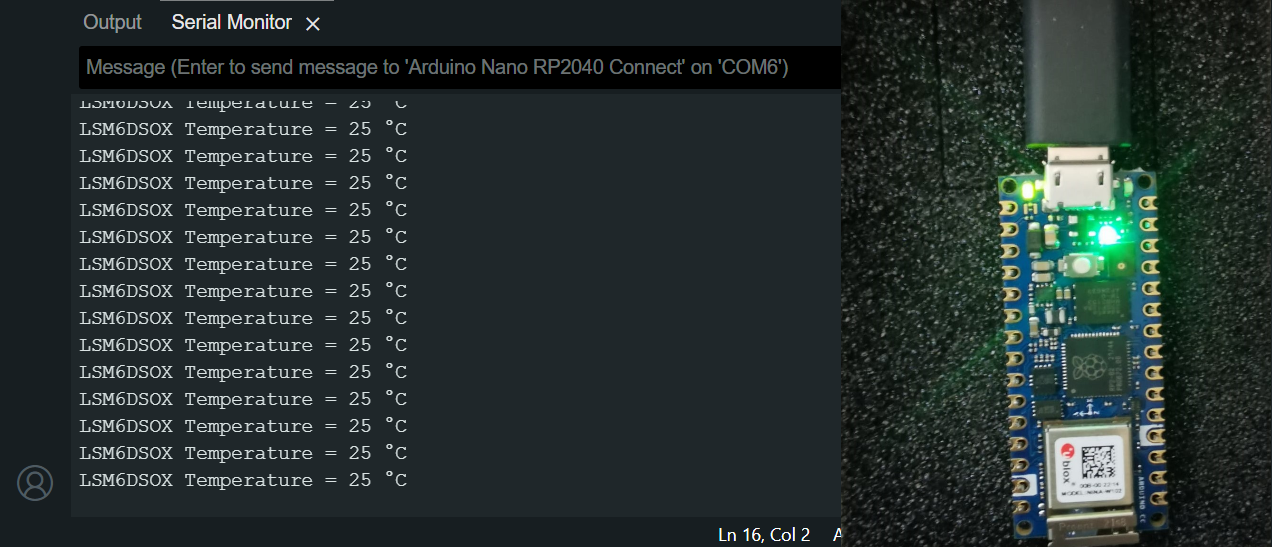
\includegraphics[width=1\textwidth]{exercise_intro/exercise2_temperature_green}
    \caption{Temperature Sensor between 20 and 36 degrees Celsius}
    \label{fig:temperature_sensor_green}
\end{figure}

\begin{figure}[h!]
  \centering
  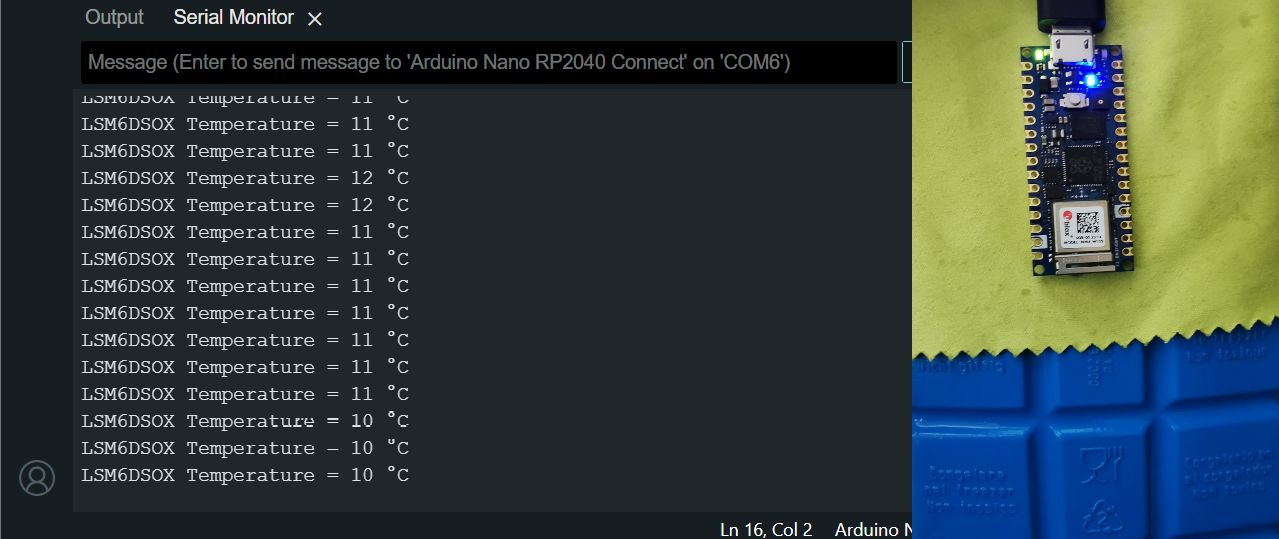
\includegraphics[width=1\textwidth]{exercise_intro/exercise2_temperature_blue}
  \caption{Temperature Sensor under 20 degrees Celsius}
  \label{fig:temperature_sensor_blue}
\end{figure}

\begin{figure}[h!]
  \centering
  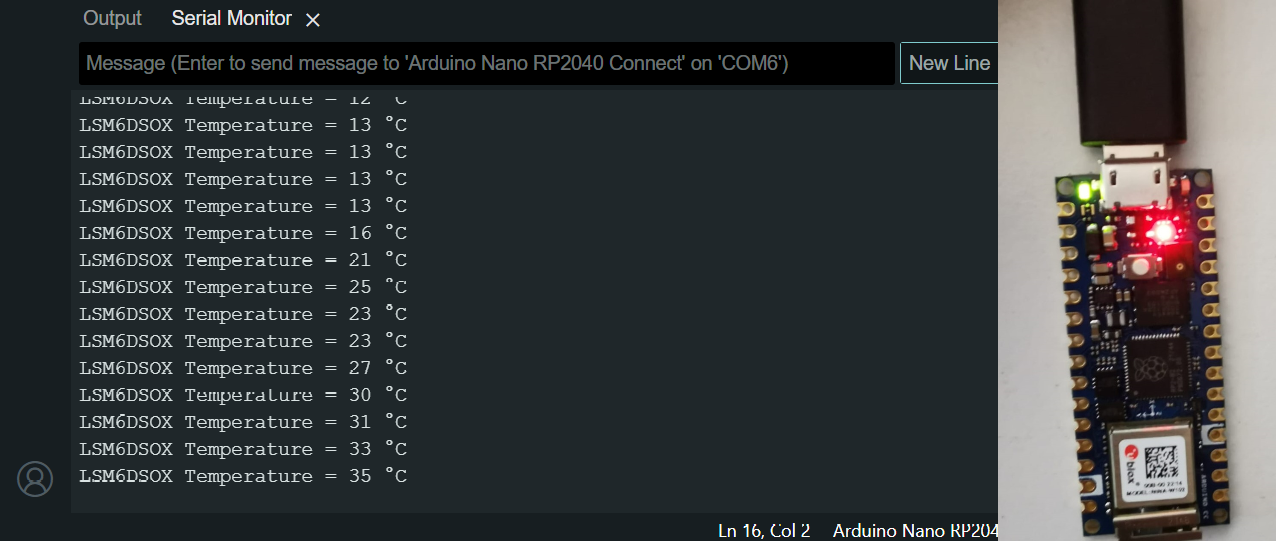
\includegraphics[width=1\textwidth]{exercise_intro/exercise2_temperature_red}
  \caption{Temperature Sensor above 36 degrees Celsius}
  \label{fig:temperature_sensor_red}
\end{figure}

\newpage

\section{Exercise 1.3: Microphone}

In the third exercise we are going to use the internal microphone to measure the sound level.
Therefore we used the link provided in the task description.
Like seen in the figures below, the LED turn on/off when a certain sound level is reached.
\newline
\newline
Like before the code for this exercise can be seen on the github repository \url{https://github.com/Smokey95/AIN_Ubiquitous_Computing/blob/main/exercise/exercise3_microphone/exercise3_microphone.ino}
It has to be noted that the \code{while-loop} for preventing the program from running till a serial monitor is connected will only work 
if all monitors are closed (even in other Arduino IDE instances).

\begin{figure}[h]
  \centering
  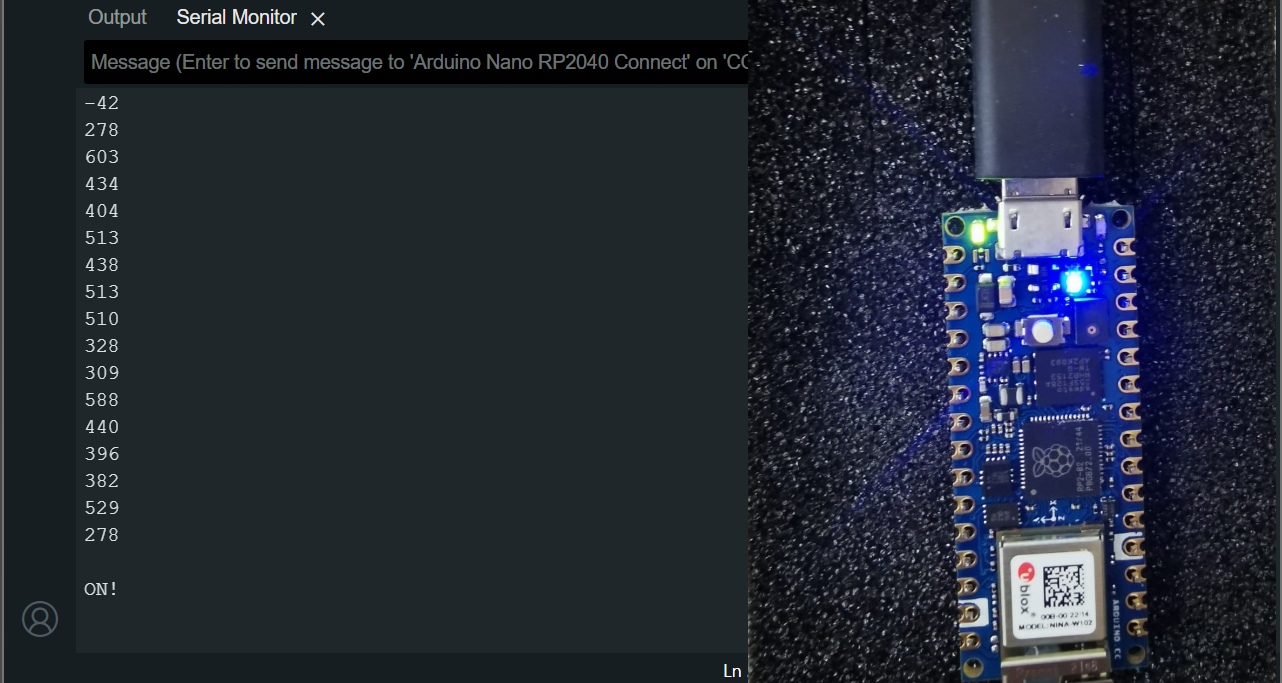
\includegraphics[width=1\textwidth]{exercise_intro/exercise3_mic_on}
  \caption{Sound detected, LED on}
  \label{fig:microphone_on}
\end{figure}

\begin{figure}[h]
  \centering
  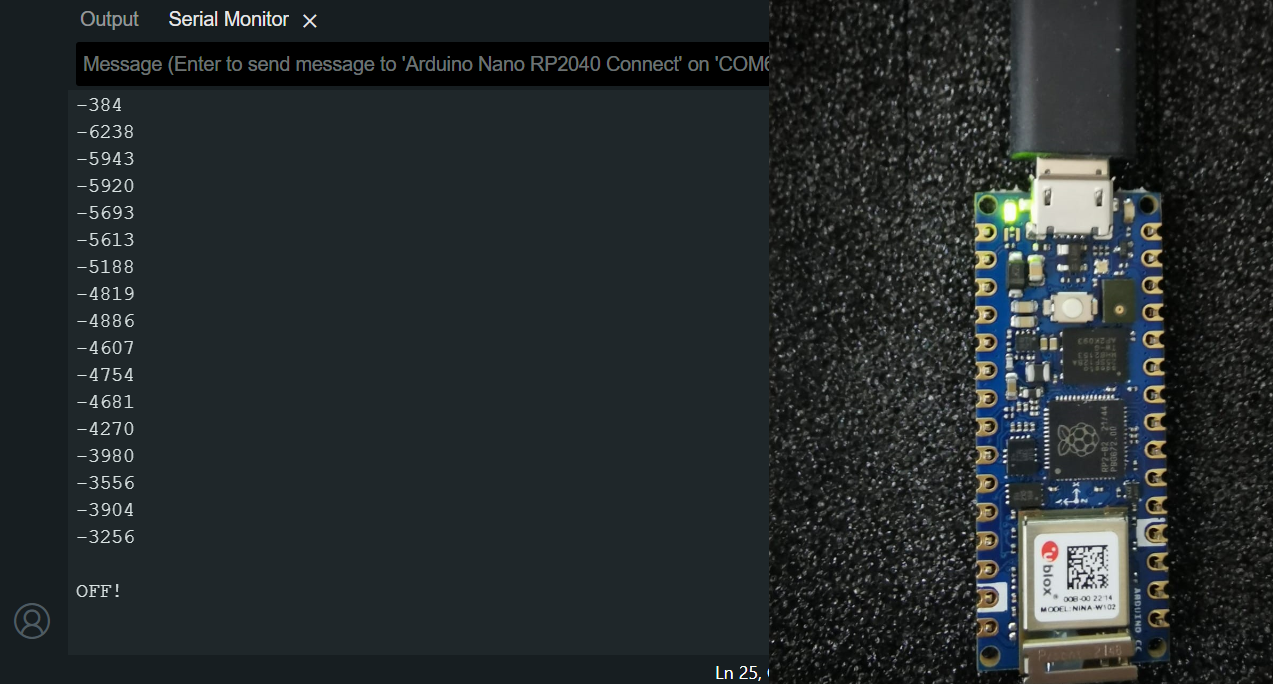
\includegraphics[width=1\textwidth]{exercise_intro/exercise3_mic_off}
  \caption{Sound detected, LED off}
  \label{fig:microphone_off}
\end{figure}


\section{Exercise 1.4: Posture Detector. Accelerometer}

In the last exercise we are going to use the internal accelerometer to detect the posture of the Arduino board.
Therefore we used the link provided in the task description to realize the following code as well as the serial monitor output seen in figure \ref{posture_detector}.
Like before the code can be seen on the github repository \url{https://github.com/Smokey95/AIN_Ubiquitous_Computing/blob/main/exercise/exercise4_posture/exercise4_posture.ino}.

\begin{figure}[h]
  \centering
  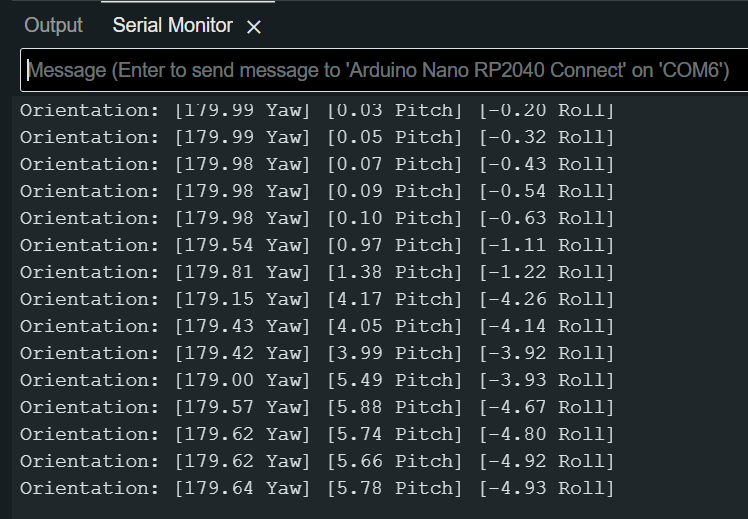
\includegraphics[width=1\textwidth]{exercise_intro/exercise_4_orientation}
  \caption{Posture Detector}
  \label{posture_detector}
\end{figure}

\chapter{Exercise 2: Node-RED}

In this exercise we will get to know the programming tool Node-RED which will be used 
for wiring together hardware devices, APIs and online services in new and interesting ways.

As the tool is primary picture based, there will not be much code in this exercise.
The exported \code{.json} of the Node-RED flow can be found in the sheet 2 folder of the 
\url{https://github.com/Smokey95/AIN_Ubiquitous_Computing} in the exercise section.


\section{Exercise 2.1; Hello World}

We will start with an basic example to get familiar with the tool b< just triggering a 
simple \code{Hello World} message.

\begin{figure}[h!]
  \centering
  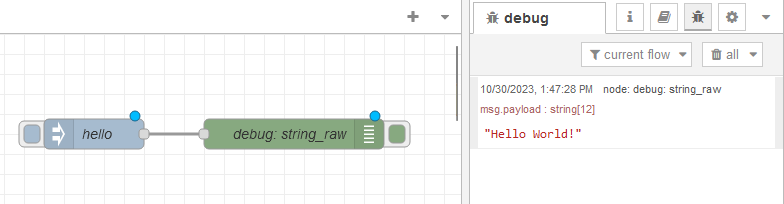
\includegraphics[width=1\textwidth]{exercise_node-red/exercise_1}
  \caption{Hello World}
  \label{fig:hello_world}
\end{figure}


\section{Exercise 2.2: Change Message}

In this exercise we will change the incoming \code{Hello World} message to \code{Hello Mars} and 
print it to the debug console.

\begin{figure}[h!]
  \centering
  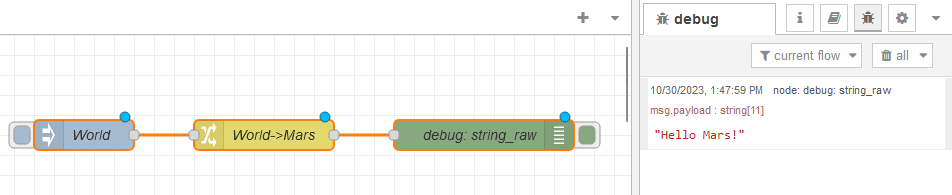
\includegraphics[width=1\textwidth]{exercise_node-red/exercise_2}
  \caption{Change Message}
  \label{fig:change_message}
\end{figure}


\section{Exercise 2.3: HTTP Request}

In this exercise we will use the \code{http request} node to get the current earthquake data from 
the \url{https://earthquake.usgs.gov/earthquakes/feed/v1.0/summary/significant_month.csv}.
It was decided to print the raw data to the debug console. Also the \code{change} node was used to 
change payload where the \code{mag} data was greater than 5.3 to \code{Panic!}.

\begin{figure}[h!]
  \centering
  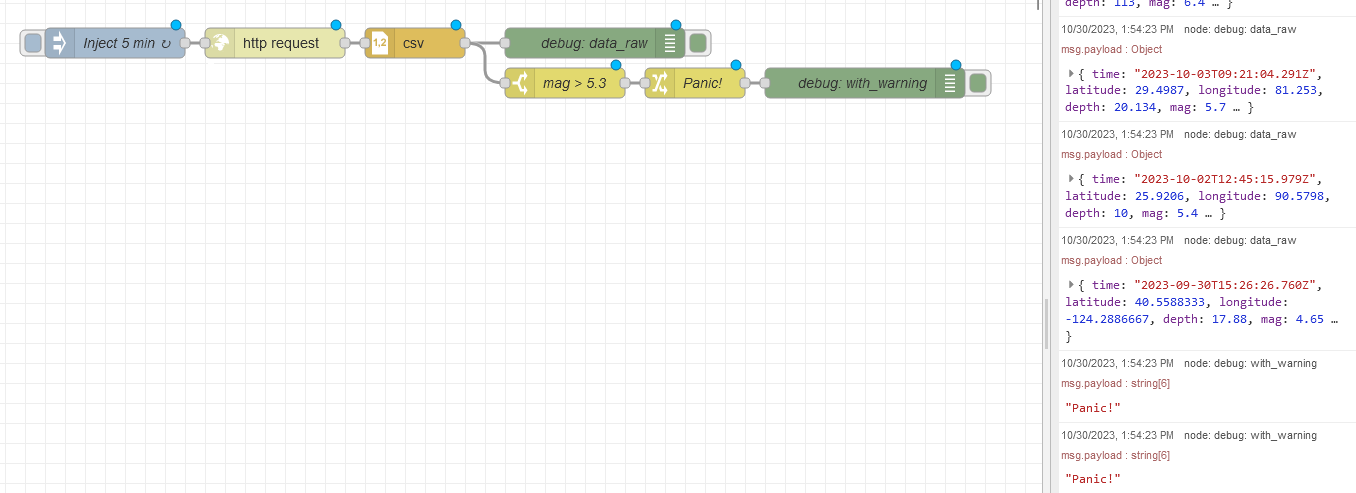
\includegraphics[width=1\textwidth]{exercise_node-red/exercise_3}
  \caption{HTTP Request}
  \label{fig:http_request}
\end{figure}


\section{Exercise 2.4: Dashboards}

In this exercise we will use the \code{dashboard} node to create a simple dashboard which will 
show the current time in several different formats.

\begin{figure}[H]
  \centering
  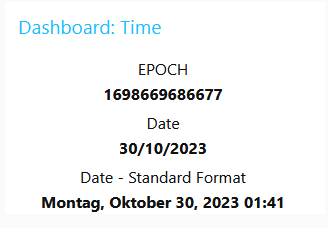
\includegraphics[width=0.8\textwidth]{exercise_node-red/exercise_4_dashboard}
  \caption{Dashboard}
  \label{fig:dashboard}
\end{figure}

\begin{figure}[H]
  \centering
  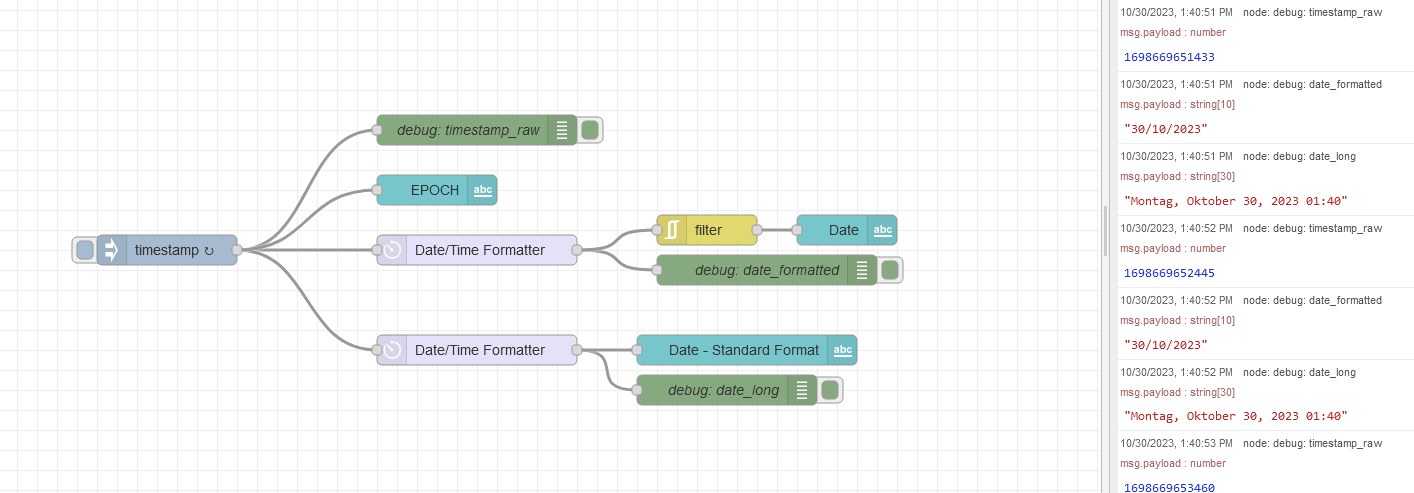
\includegraphics[width=1\textwidth]{exercise_node-red/exercise_4_node}
  \caption{Nodes}
  \label{fig:4_nodes}
\end{figure}

To display the date with written day name and month some time were spent to find the correct 
formatting of \code{dddd, MMMM DD, YYYY hh:mm} to display the timestamp like wanted.


\section{Exercise 2.5: LED Control}

In the fifth exercise we will use the \code{led} node to control the LED on the Arduino board as 
well as a hardware setup like seen [here](https://docs.arduino.cc/built-in-examples/digital/Button).

Notable is that instead of using the \code{5V} pin to power the LED, the \code{3.3V} pin was used 
cause even when operating the circuit with an pull down resistor the \code{5V} signal was bouncing.
Instead working with the \code{3.3V} signal was like expected.

The code below running on the Arduino board is as simple as expected.

\begin{minted}
  [
    frame=lines,
    framesep=2mm,
    baselinestretch=1.2,
    linenos
  ]
  {C}

  #include <WiFiNINA.h>

  const int button_pin = 4;
  
  void setup() {
    // Initalize LEDs
    pinMode(LEDR, OUTPUT);
  
    // initialize the pushbutton pin
    pinMode(button_pin, INPUT);
  
    Serial.begin(9600);
  }
  
  void loop() {
  
    static int debounce = 0;
    static String msg = "";
  
    // put main code here, to run repeatedly:
  
    if (Serial.available() > 0) {
      msg = Serial.readString();
    }
  
    if (digitalRead(button_pin) == HIGH || 
        msg.compareTo("1") == false){
      digitalWrite(LEDR, HIGH);       // Red LED on
      Serial.println(1);              // Writeback status for dashboard
    } else {
      digitalWrite(LEDR, LOW);        // Red LED off
      Serial.println(0);
    }
    
    delay(100);
  }
\end{minted}

The figure below shows the Node-RED flow with the hardware button on the breadboard pushed (notable 
cause software button is not pushed but LED is on) and the dashboard showing the correct status.

\begin{figure}[H]
  \centering
  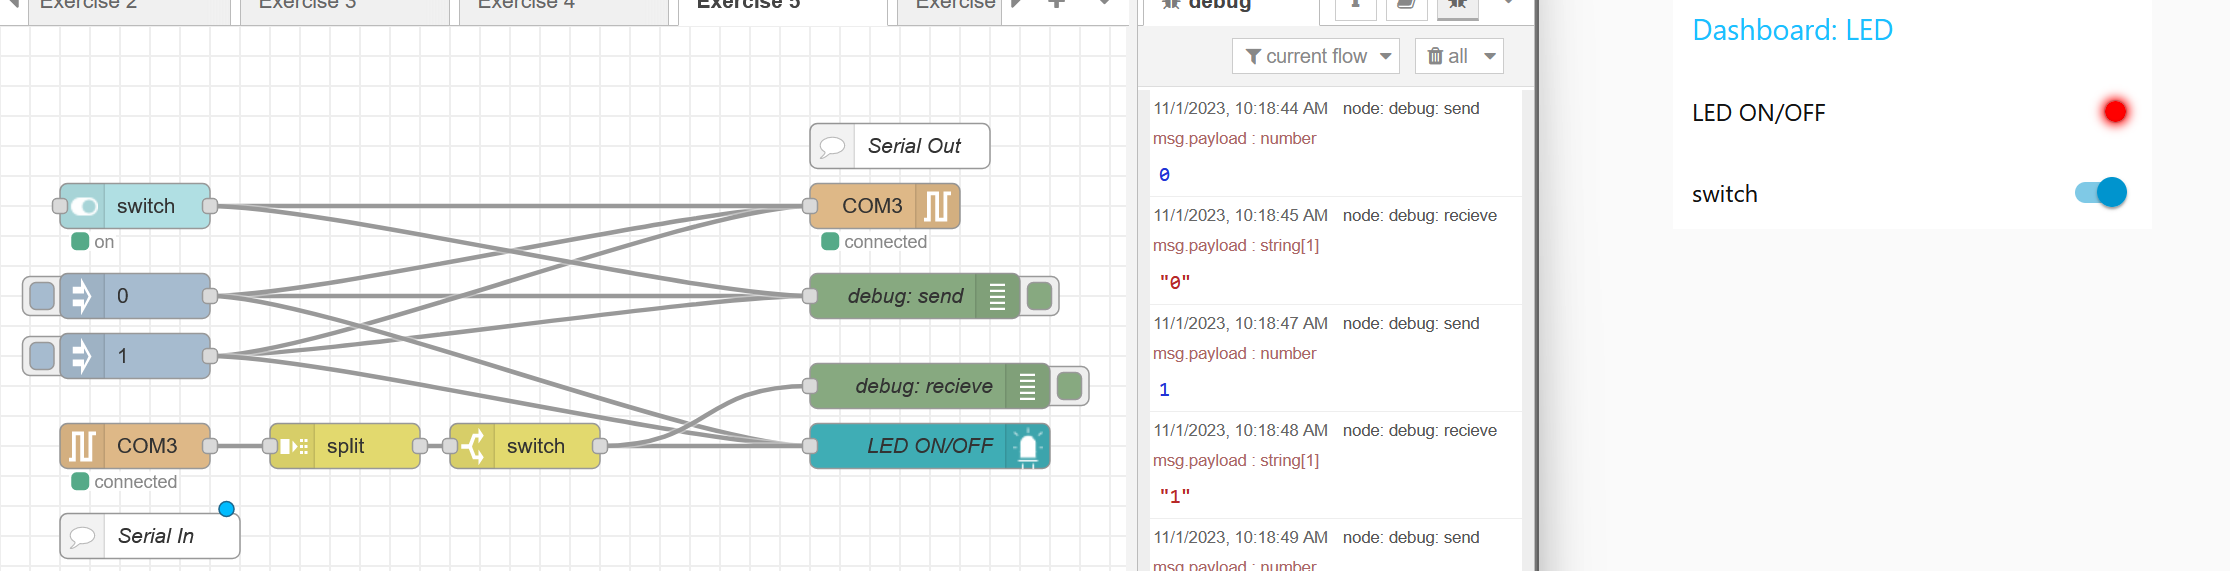
\includegraphics[width=1\textwidth]{exercise_node-red/exercise_5}
  \caption{LED Control}
  \label{fig:led_control}
\end{figure}


\section{Exercise 2.6: Temperature}

In this exercise we will use the \code{gauge} node to display the current temperature of the 
Arduino board. The temperature is measured using the internal temperature sensor of the Arduino. 
It was not a requirement but i tried to reuse the code from the first exercise with no changes 
leading to expanded node red flow.

\begin{figure}[H]
  \centering
  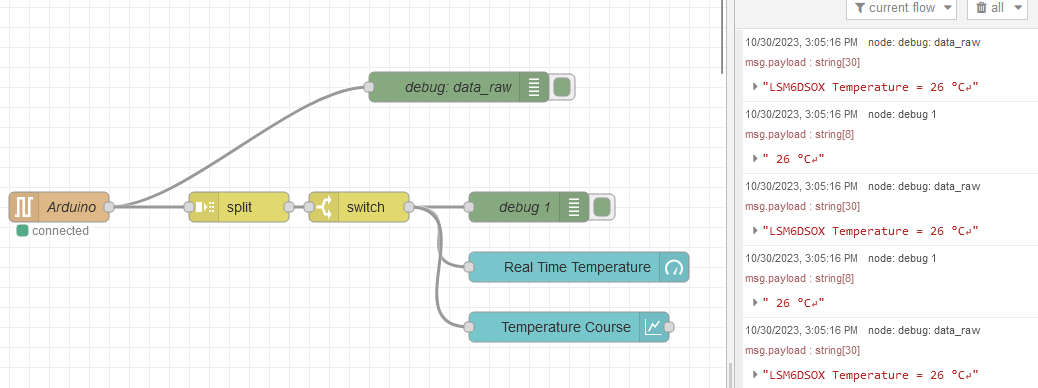
\includegraphics[width=1\textwidth]{exercise_node-red/exercise_6_full}
  \caption{Temperature}
  \label{fig:temperature}
\end{figure}

Like seen in the figure above, the Arduino board prints the current temperature to the serial port 
like in the code from the first exercise. To process this data the \code{split} node was used to 
split the incoming data stream and a \code{switch} node which will compare incoming data if it 
\code{contains °C} and only forward this data.

The resulting dashboard can be seen in the figure below.

\begin{figure}[H]
  \centering
  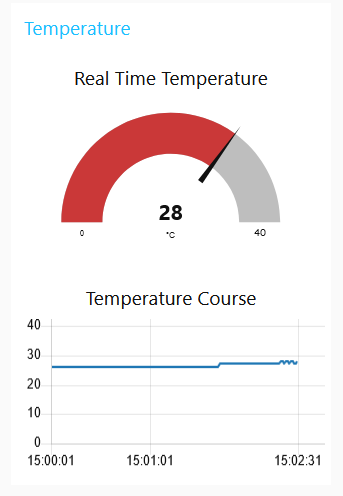
\includegraphics[width=0.5\textwidth]{exercise_node-red/exercise_6_dashboard}
  \caption{Temperature Dashboard}
  \label{fig:temperature_dashboard}
\end{figure}


\section{Exercise 2.7: MQTT}

In this exercise we will use the \code{mqtt} node to send the current temperature to a MQTT broker 
(hosted on \url{https://www.hivemq.com/try-out/}) and display it on a dashboard 
on \url{https://www.datacake.de/}.

Most effort was spent on this exercise cause it was not clearly described (or at least for me) 
how important the \code{topic} field is. This field has to match either in Node-RED config 
as well as on the datacake settings. Even after figure this out the data was not processed 
right so i created a second flow which send the data to the broker where it will be 
returned as \code{raw\_data}.

Also it has to be noted that this time the code of the Arduino was changed to send the 
temperature in a json styled format to the serial port. As most of the code was not changed 
only the relevant part is shown below.

\begin{minted}
  [
    frame=lines,
    framesep=2mm,
    baselinestretch=1.2,
    linenos
  ]
  {C}

  ...
  // Offset of ~30%
  float temperature_normalized = temperature_deg / 1.3;

  // Create a JSON-formatted string
  String jsonString = "{\"temp\": " + String(temperature_normalized) + "}";

  // Send JSON-formatted string over serial
  Serial.println(jsonString);
  ...

\end{minted}

This data will then rooted from the serial port to the \code{mqtt} node which will send it to 
the broker. Notice that the data will be send to two different topics. One topic is used to 
send data to an raw channel and the other one is used to send data to a formatted channel (see 
figure below).

\begin{figure}[H]
  \centering
  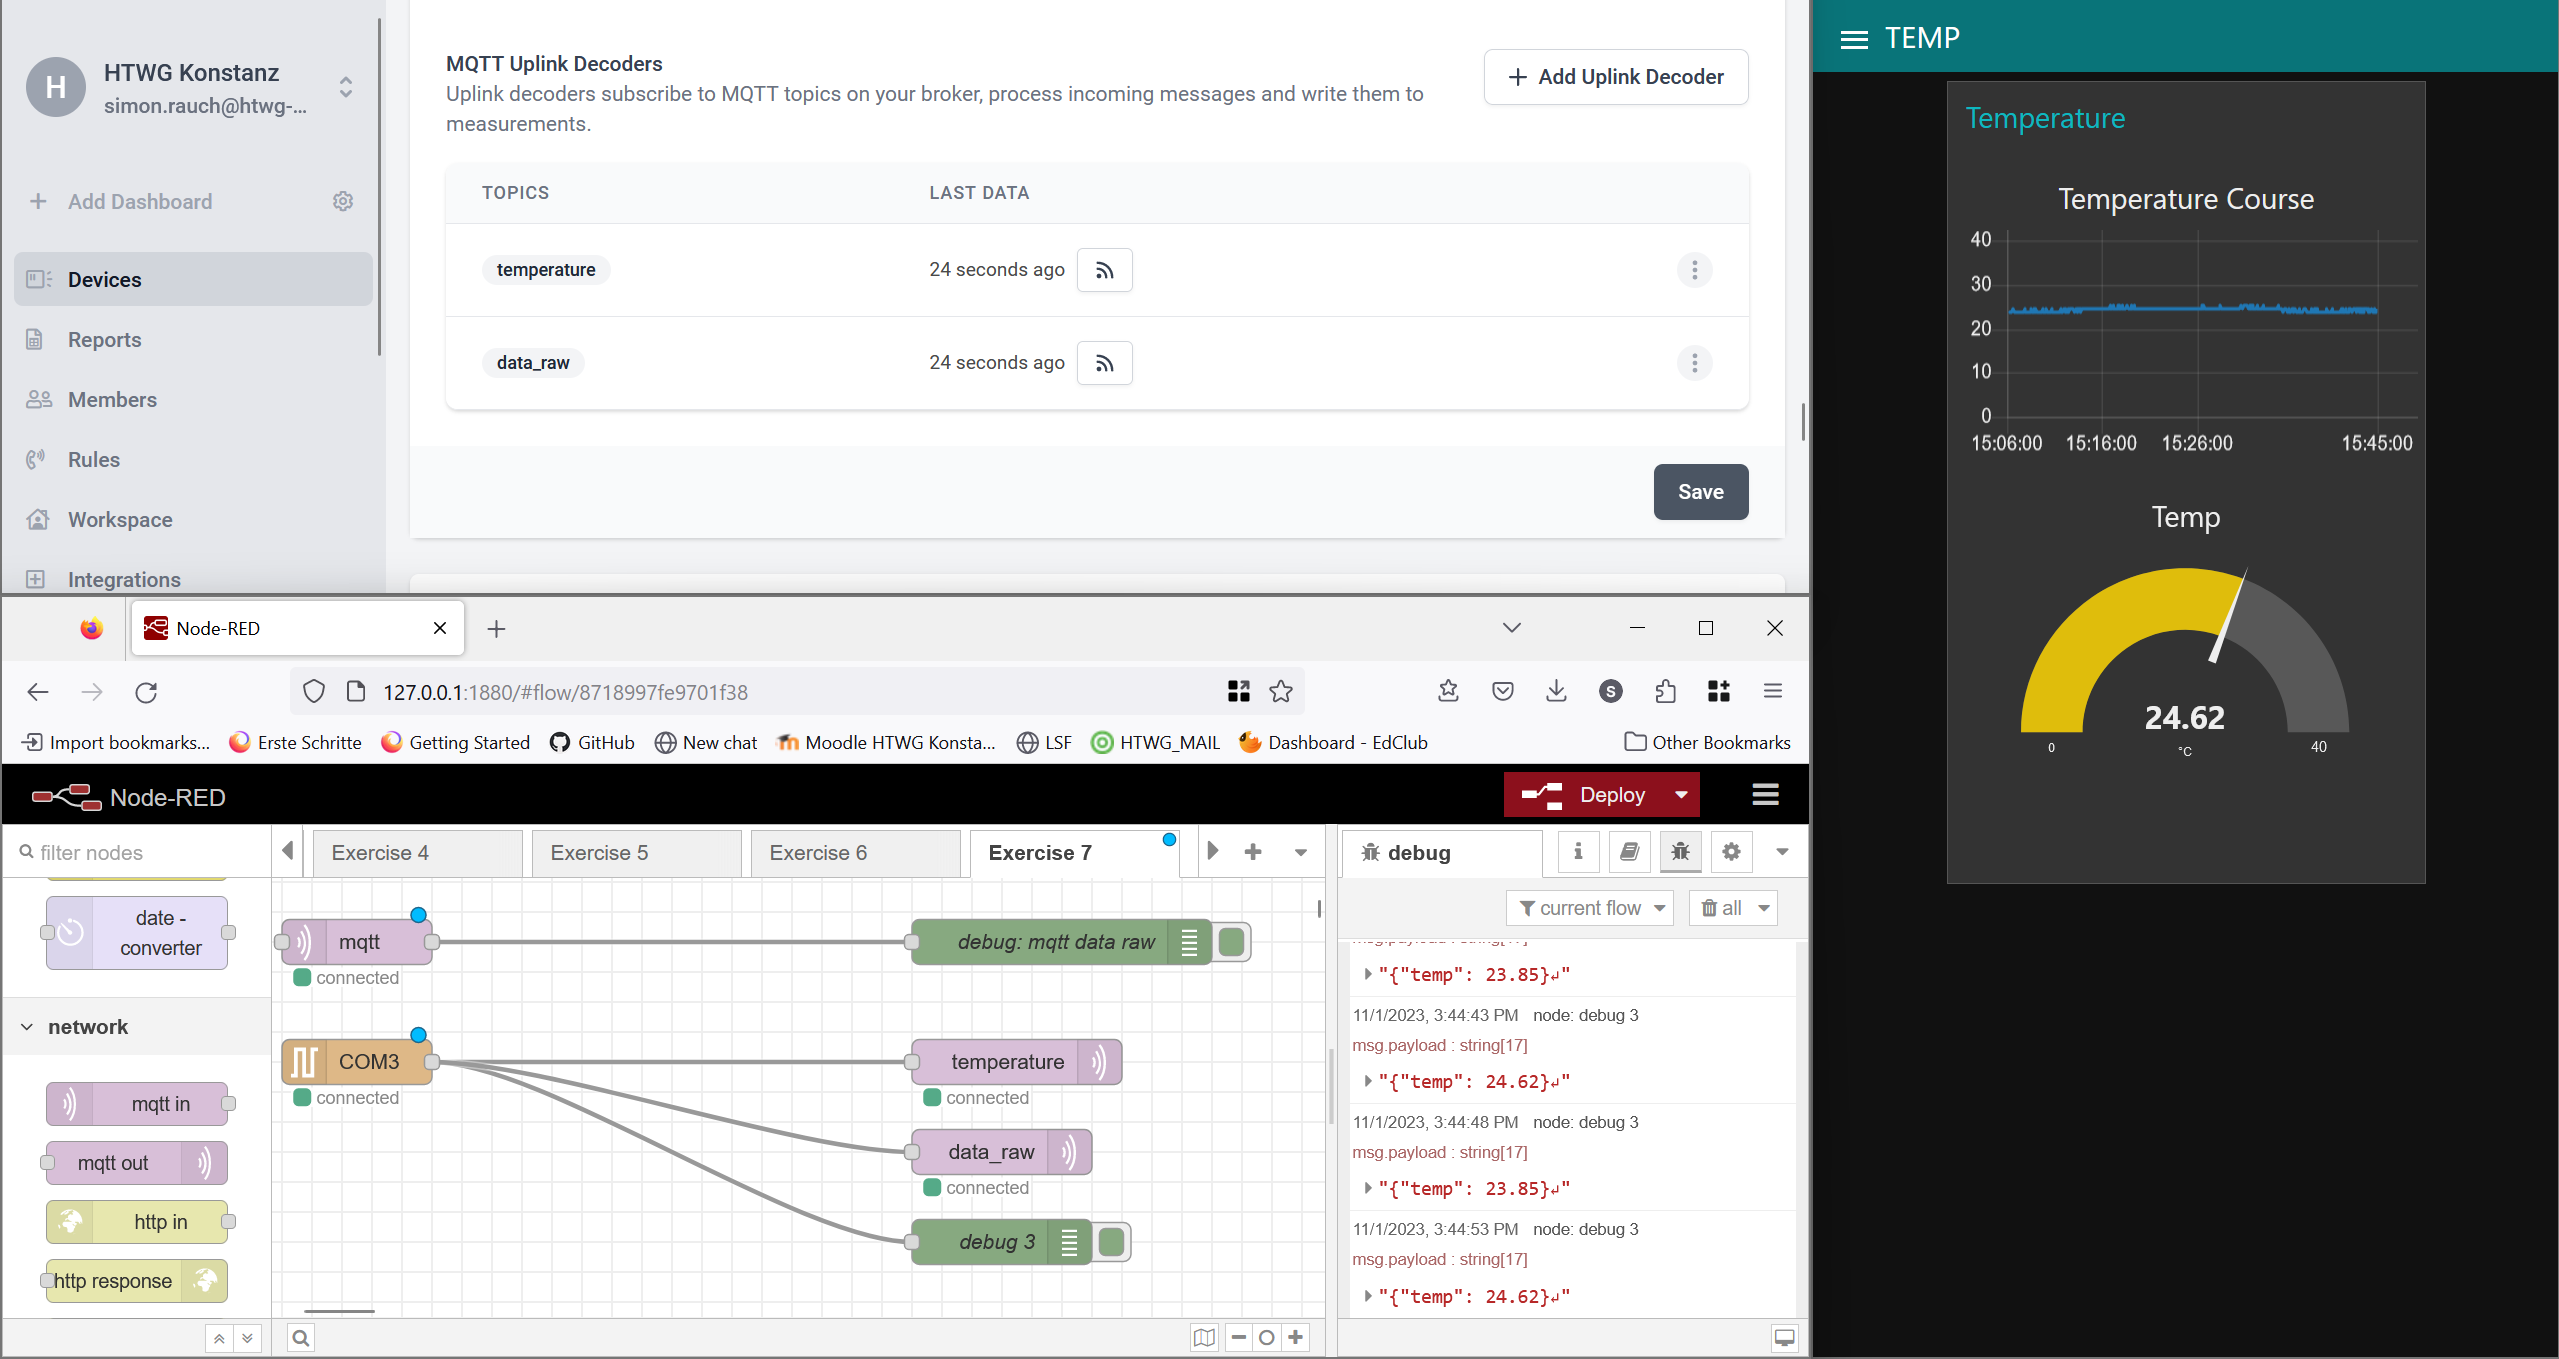
\includegraphics[width=1\textwidth]{exercise_node-red/exercise_7_data_raw}
  \caption{MQTT}
  \label{fig:mqtt}
\end{figure}

I spent some more time cause i does not why but even if the same data was send to both topics 
only the raw data was seen on datacake even if both Uplink decoder were the same. 
To waste no more time the decoder from the temperature channel was moved to the raw channel 
which worked fine and data was displayed on the dashboard.
Following you will see the java script to parse the data from the raw channel to the temperature field 
as well as the dashboard.

\begin{minted}
  [
    frame=lines,
    framesep=2mm,
    baselinestretch=1.2,
    linenos
  ]
  {javascript}

  function Decoder(topic, payload) {
    // Transform incoming payload to JSON
    payload = JSON.parse(payload);
    
    // Extract Temperature from payload, do calculation
    var temperature = payload.temp;
    
    // Forward Data to Datacake Device API using Serial, Field-Identifier
    return [
        {
            device: "e8aec33d-a641-4d25-a235-786fd1291a7b", // Serial Number or Device ID
            field: "TEMPERATURE",
            value: temperature
        },
    ];
  }
\end{minted}

\begin{figure}[H]
  \centering
  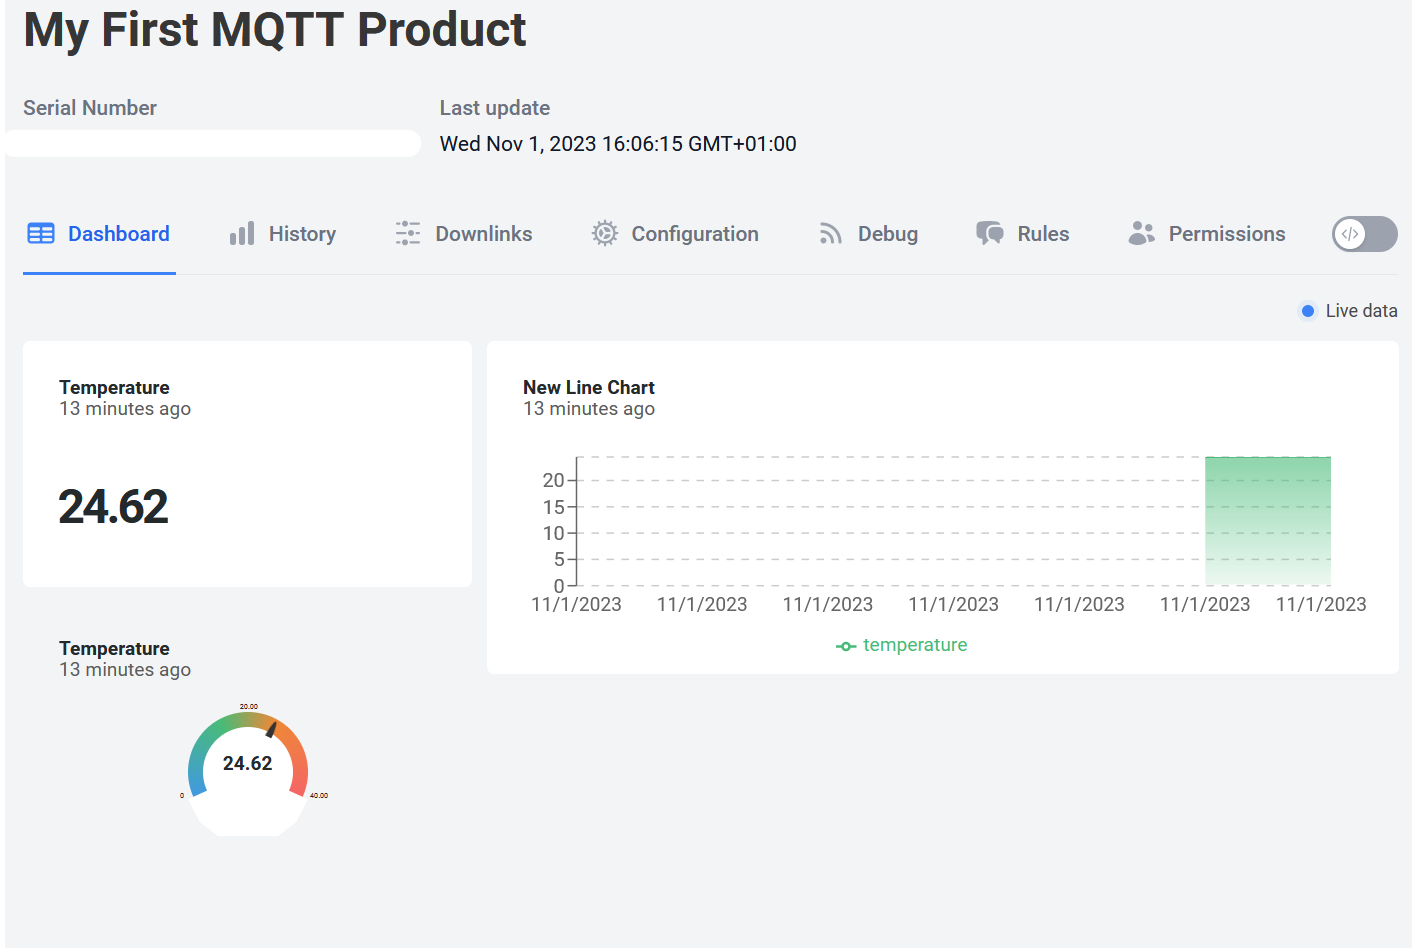
\includegraphics[width=0.8\textwidth]{exercise_node-red/exercise_7_dashboard}
  \caption{MQTT Dashboard}
  \label{fig:mqtt_dashboard}
\end{figure}

At the end of this exercise a downlink was setup to send a message to the Arduino board.
This was also a little bit frustrating but the config as well as the result can be seen below.

\begin{figure}[H]
  \centering
  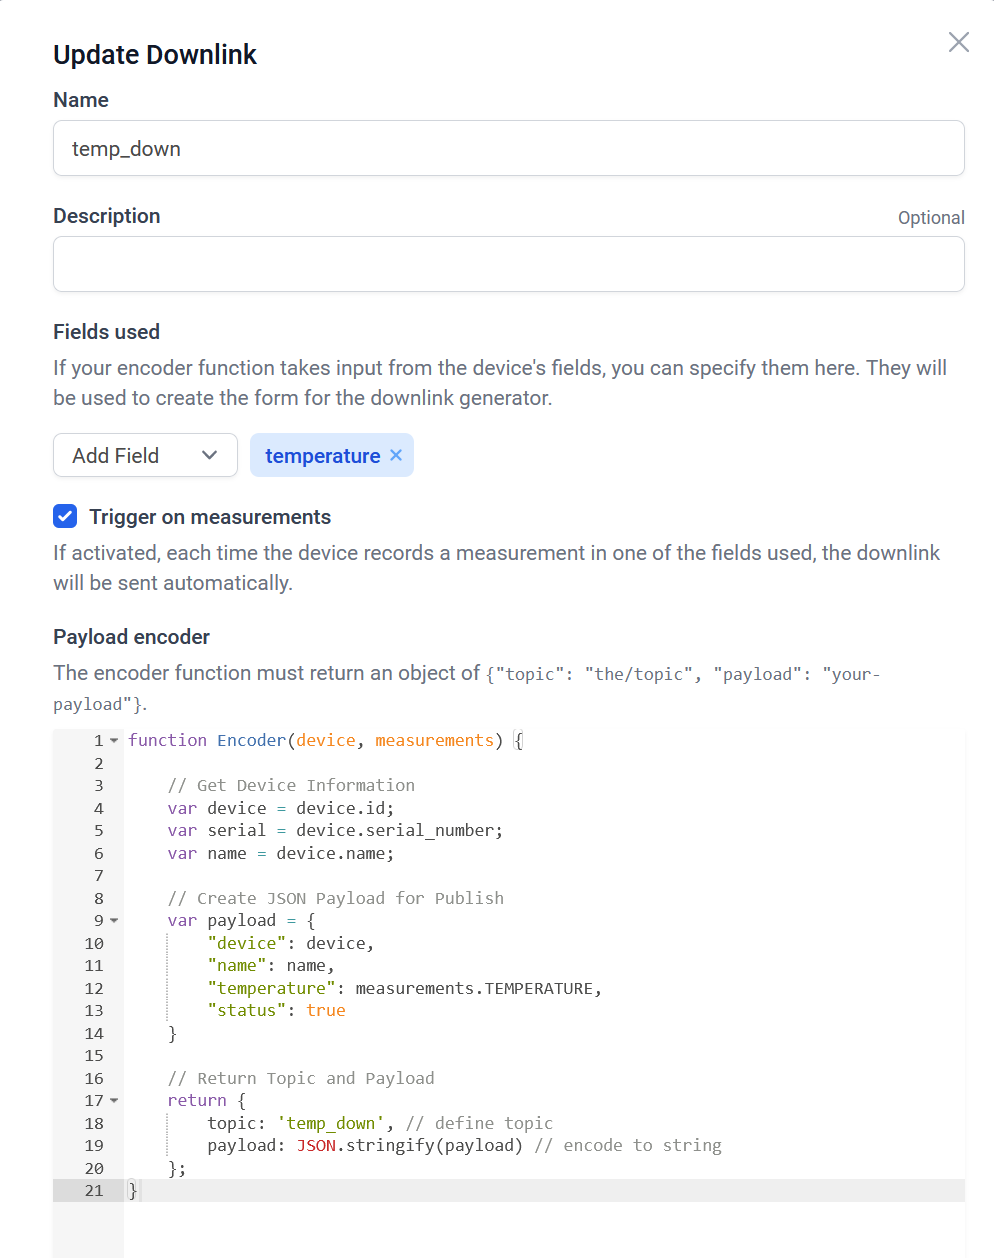
\includegraphics[width=0.7\textwidth]{exercise_node-red/exercise_7_downlink}
  \caption{MQTT Downlink}
  \label{fig:mqtt_downlink}
\end{figure}

\begin{figure}[H]
  \centering
  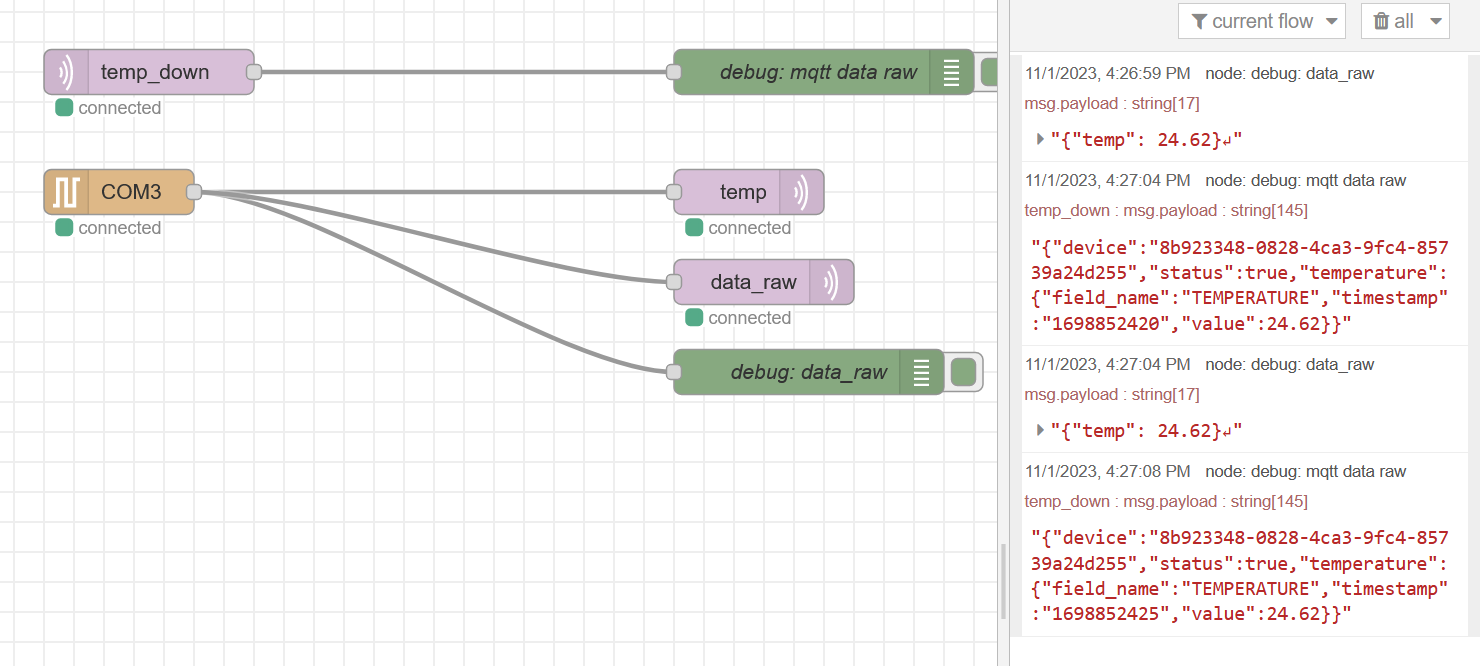
\includegraphics[width=0.8\textwidth]{exercise_node-red/exercise_7_data_down}
  \caption{MQTT Downlink Result}
  \label{fig:exercise_7_data_down}
\end{figure}


\section{Exercise 2.8: Cat door}

In the last exercise we will use the \code{mqtt} as well as the arduinos \code{gyroscope} to 
detect if the cat door is open or closed. The gyroscope is used to detect the angle of the door 
as well as the direction it is opened (detecting if cat is indoor or outdoor).
\newline
\newline
The code running on the arduino board is shown below.

\begin{minted}
  [
    frame=lines,
    framesep=2mm,
    baselinestretch=1.2,
    linenos
  ]
  {C}

  #include <WiFiNINA.h>
  #include <Arduino_LSM6DSOX.h>
  #include <MadgwickAHRS.h>

  Madgwick filter;

  void setup() {
    // Initialize serial communication and wait for port to open:
    Serial.begin(9600);
    while (!Serial) {
      ; // wait for serial port to connect. Needed for native USB port only
    }

    // Initialize the LSM6DSOX
    if (!IMU.begin()) {
      Serial.println("Failed to initialize IMU!");
      while (1);
    }

    filter.begin(104.00);

    // Initalize LEDs
    pinMode(LEDR, OUTPUT);
    pinMode(LEDG, OUTPUT);
    pinMode(LEDB, OUTPUT);

    digitalWrite(LEDR, LOW);    // Red
  }

  void loop() {
    float ax, ay, az;
    float gx, gy, gz;
    static int counter = 0;
    static bool state;
    static float temp = 0;

    // check if data is available every loop
    if(IMU.accelerationAvailable() && 
       IMU.gyroscopeAvailable()) {

      IMU.readAcceleration(ax, ay, az);
      IMU.readGyroscope(gx, gy, gz);

      // Update the filter with the latest data
      filter.updateIMU(gx, gy, gz, ax, ay, az);

      // Check the filter's roll for door movement
      if (filter.getRoll() > 5){
        state = true;
        digitalWrite(LEDR, HIGH); // Turn on LED if door is opened
      } else if (filter.getRoll() < -5) {
        state = false;
        digitalWrite(LEDR, HIGH); // Turn on LED if door is opened
      } else {
        digitalWrite(LEDR, LOW); // Turn off LED if door is closed
      }
    }

    if(!(counter % 100)){
      temp = get_temp();
      send_data(temp, state);
    }

    counter > 100 ? counter = 1 : counter++;
    delay(100);
  }

  float get_temp() {
    // Check if temperature is available
    if (IMU.temperatureAvailable())
    {
      int temperature_deg = 0;
      IMU.readTemperature(temperature_deg);

      // Offset of ~30%
      float temperature_normalized = temperature_deg / 1.3;

      return temperature_normalized;
    }
  }

  void send_data(float temp, bool in_out){
    // Construct JSON-style string
    String jsonString = "{\"temperature\": " + String(temp) + ", \"state\": \"" + (in_out ? "outdoor" : "indoor") + "\"}";
    Serial.println(jsonString);
  }

\end{minted}

Note that the sensor is checked in every iteration but the data is only send every 100th iteration to reduce 
the amount of data send to the broker. Also the data is send in a json styled format to the serial port.
\newline
\newline
Like seen in in the figure below the data is then send to the broker using \code{Node\-RED} where it is 
collected and displayed from \code{datacake}.

\begin{figure}[H]
  \centering
  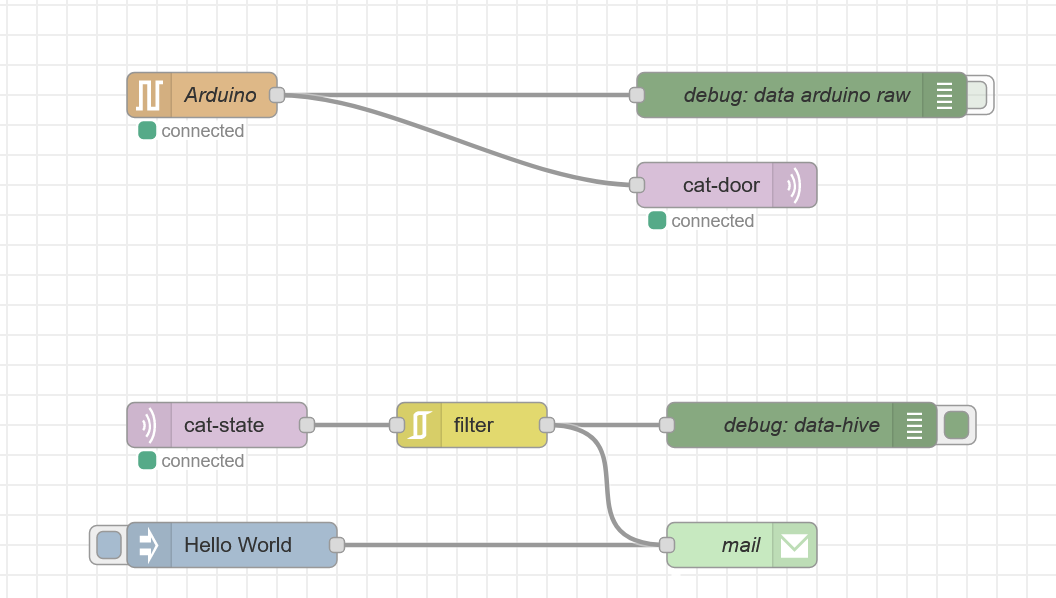
\includegraphics[width=1\textwidth]{exercise_node-red/exercise_8_node-red}
  \caption{Cat Door Note-RED Flow}
  \label{fig:cat_door}
\end{figure}

Also the data is send back from \code{datacake} to the \code{Note\-RED} flow using the \code{Downlink} feature 
which was introduced in the last exercise. This will trigger a \code{Mail} node which will send an email to 
the configured email address. (Cause of privacy reasons the \code{.json} file is not included in the repository 
cause it contains the email address.)

\begin{figure}[H]
  \centering
  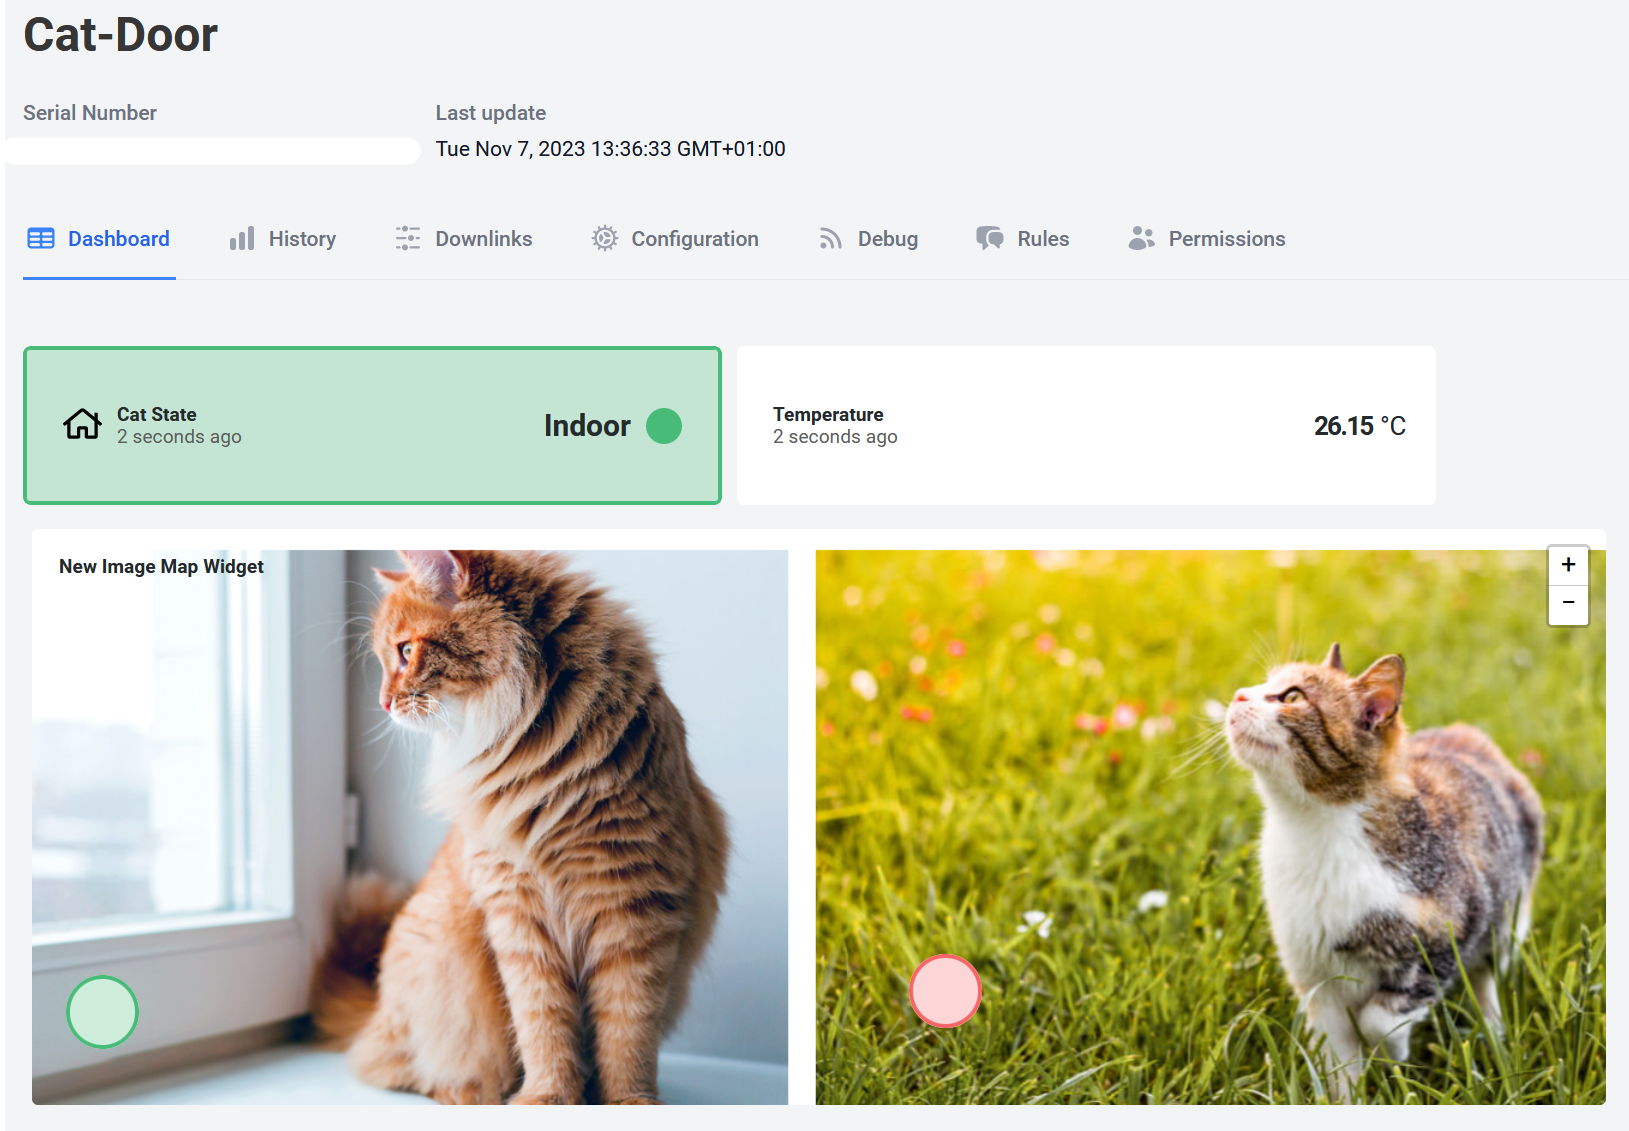
\includegraphics[width=1\textwidth]{exercise_node-red/exercise_8_dashboard}
  \caption{Cat Door Datacake}
  \label{fig:cat_door_datacake}
\end{figure}

\chapter{Exercise 3: MicroPython}
\section{Exercise 3.1: Creating a Cumulocity IoT Student Account}
So the first was to create a Cumulocity IoT Student Account which might be straight forward but due to 
a outdated exercise description it was not that easy cause the link to the Cumulocity platform was deprecated.
Anyway after finding the way to the Cumulocity IoT page the default dashboard was shown. At this point I am 
not completely sure if there is a need to do this exercise using a new platform or why it is not possible to 
use \code{datacake} which was used in the previous exercise.


\section{Exercise 3.2 Setup}
So setup for this exercise was a real pain an unfortunately the exercise description did not help at all.
The first problem was to even get a working connection to the board via USB to install \code{micropython}.
After installing \code{Thonny} the device were not shown like described further more the 
suggested \code{Arduino Micropython Tools} from Arduino which can be found \href{https://labs.arduino.cc/en}{\textit{here}} 
did not work at all. After some research I found a working solution with \code{Thonny} (see pictures below).
It is highly recommended from my side to update this exercise description and give hints about setting device 
in Bootloader-Mode etc.
\newline
\newline
So the following steps were done to get a working connection to the board:
\begin{enumerate}
  \item Download and install \code{Thonny} from [here](https://thonny.org/)
  \item Open \code{Thonny} and connect the board via USB
  \item Click on \code{Local Python 3} in the upper right corner and select \code{Configure Interpreter}
        \begin{figure}[H]
          \centering
          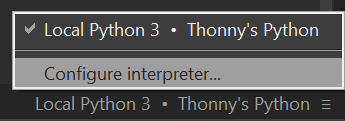
\includegraphics[width=0.6\textwidth]{exercise_micro-python/configure_interpreter.png}
          \caption{Thonny - Configure Interpreter}
        \end{figure}
  \item Select \code{MicroPython(RP2040)} and select the correct port
        \begin{figure}[H]
          \centering
          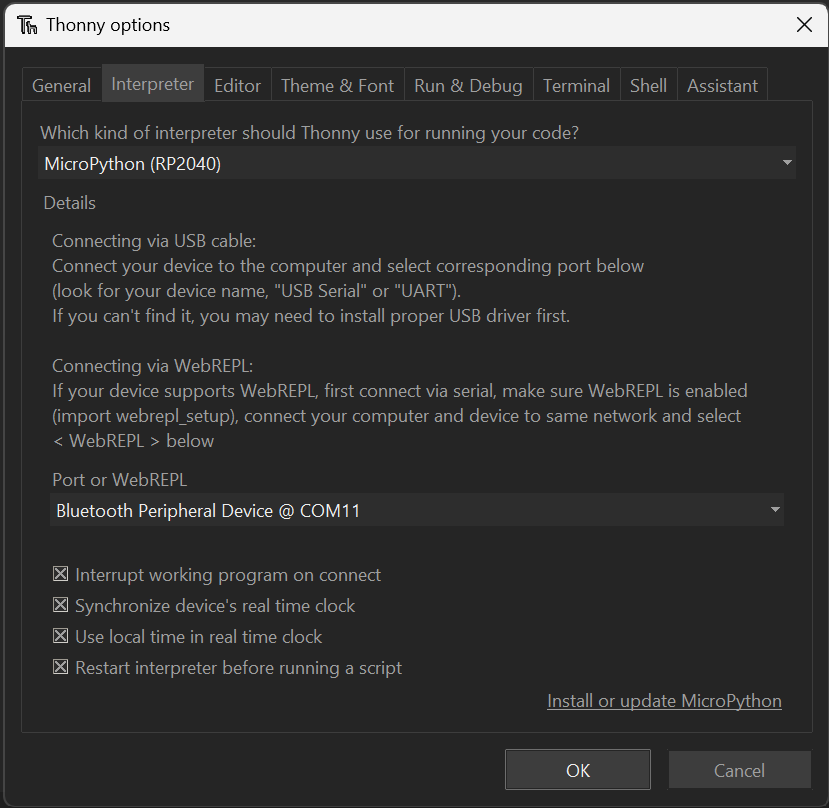
\includegraphics[width=0.6\textwidth]{exercise_micro-python/configure_device.png}
          \caption{Thonny - Select Interpreter}
        \end{figure}
  \item Click on \code{Install or update MicroPython}
  \item Select the target settings like shown in the picture below
        \begin{figure}[H]
          \centering
          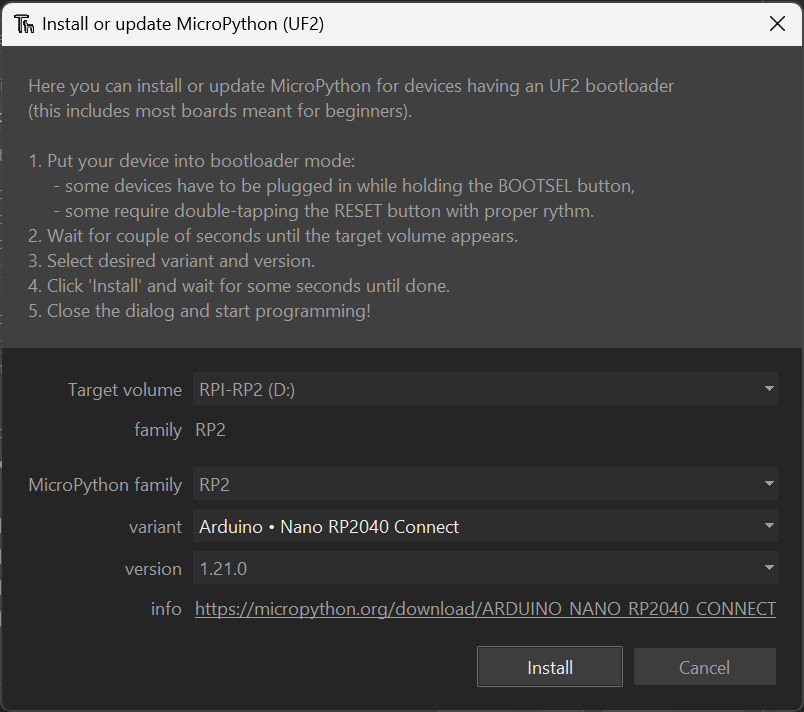
\includegraphics[width=0.6\textwidth]{exercise_micro-python/configure_micro_python.png}
          \caption{Thonny - Install MicroPython}
        \end{figure}
  \item NOTE: In some cases it is necessary to set the board in Bootloader-Mode by pressing \code{Reset} button twice
\end{enumerate}

To test if the installation was successful I used the following code to blink the LED on the board which 
could be found \href{https://forum.arduino.cc/t/blinking-the-rgb-lights-in-micropython/868974}{\textit{here}}:
As this example is very huge I wrote a small script inspired by Arduino page \href{https://docs.arduino.cc/micropython/basics/digital-analog-pins}{\textit{here}}.
The code could be seen bellow, it just blinks the LED connected to PIN 25 on the board.

\begin{minted}
  [
    frame=lines,
    framesep=2mm,
    baselinestretch=1.2,
    linenos
  ]
  {python}
  
  from machine import Pin
  import time

  myLED = Pin(25, Pin.OUT) #Nano RP2040 Connect
  #myLED = Pin(10, Pin.OUT) #Nano 33 BLE / Nano 33 BLE Sense
  #myLED = Pin(2, Pin.OUT) #Portenta H7


  while True:
      print("LED ON")
      myLED.value(0)
      time.sleep(1)
      print("LED OFF")
      myLED.value(1)
      time.sleep(1)
\end{minted}


\subsection{Problem with \code{network} module}

After installing \code{micropython} on the board I tried to connect to the WiFi using the following code which 
could be found \href{https://docs.arduino.cc/micropython/basics/installing-modules}{\textit{here}}:

\begin{minted}
  [
    frame=lines,
    framesep=2mm,
    baselinestretch=1.2,
    linenos
  ]
  {python}
  
  import network

  WIFI_NETWORK='YOUR_NETWORK_NAME'
  WIFI_PASSWORD='YOUR_NETWORK_PASSWORD'

  wlan = network.WLAN(network.STA_IF)
  wlan.active(True)
  wlan.connect(WIFI_NETWORK, WIFI_PASSWORD)

  print()
  print("Connected to ",WIFI_NETWORK)
\end{minted}

This code is also part of the exercise but running this will lead to the following error:

\begin{figure}[H]
  \centering
  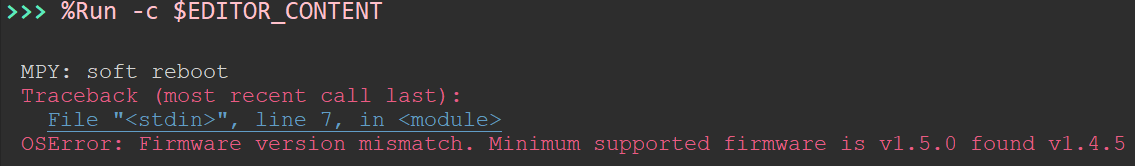
\includegraphics[width=1\textwidth]{exercise_micro-python/network_module_error.png}
  \caption{Error: Network Modul}
\end{figure}

After some research I found out that the \code{network} module is part of the \code{micropython} installation 
and this error is more or less a bug in the \code{micropython} installation. 
Research showed that there is an GitHub issue for this problem which could be found \href{https://github.com/micropython/micropython/issues/8896}{\textit{here}}.
which is still open and the workaround described there is not working for me.
There were several attempts to get this running by flashing the firmware using several tools.
It was flashed using \code{Thonny} and \code{MicroPython Installer} which is a Arduino tool 
which could be found \href{https://labs.arduino.cc/en/labs/micropython-installer/}{\textit{here}}. 
Also it was tested using \code{OpenMV} like described \href{https://docs.arduino.cc/tutorials/nano-rp2040-connect/rp2040-openmv-setup}{\textit{here}}.
Unfortunately none of these attempts were successful and the error still occurs.
Even joining \code{micropythons} Discord channel showed that there is not even a question about this problem.
\newline
\newline
At the end I decided to flash firmware manual to the device like described \href{https://micropython.org/download/ARDUINO_NANO_RP2040_CONNECT/}{\textit{here}}.
This site provides several firmware versions like shown in the image bellow:

\begin{figure}[H]
  \centering
  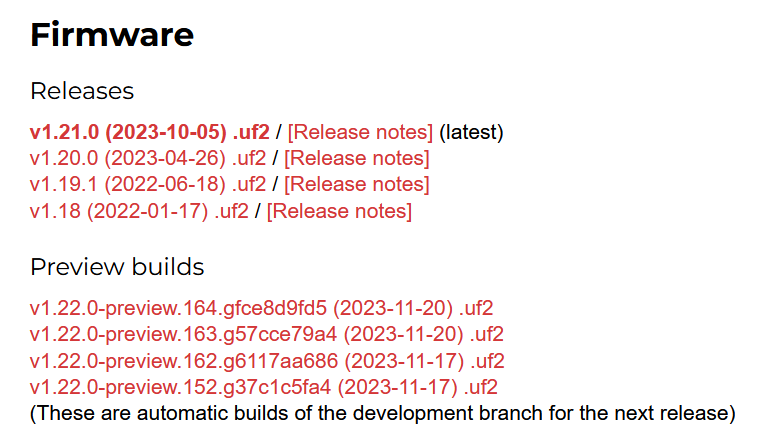
\includegraphics[width=1\textwidth]{exercise_micro-python/firmware_versions.png}
  \caption{Firmware Versions}
\end{figure}

\subsection{Flashing firmware manually}

To flash the firmware manually the following steps were done:
\begin{enumerate}
  \item Download the latest firmware version from \href{https://micropython.org/download/ARDUINO_NANO_RP2040_CONNECT/}{\textit{here}}
  \item Set device in Bootloader-Mode by pressing \code{Reset} button twice. If the device is in Bootloader-Mode the device will open as a new drive like seen bellow:
        \begin{figure}[H]
          \centering
          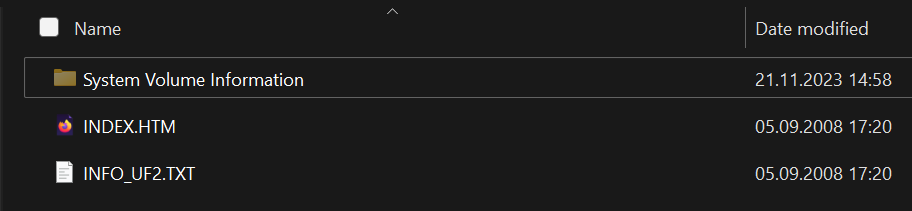
\includegraphics[width=0.6\textwidth]{exercise_micro-python/bootloader_mode.png}
          \caption{Bootloader-Mode}
        \end{figure}
  \item \textbf{Note: } If the device is open as a new drive as shown bellow it is \textbf{NOT} in Bootloader-Mode
        \begin{figure}[H]
          \centering
          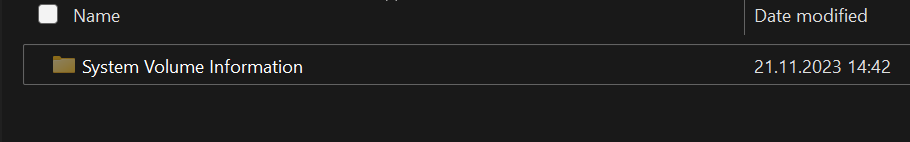
\includegraphics[width=0.6\textwidth]{exercise_micro-python/not_in_bootmode.png}
          \caption{Bootloader-Mode}
          \label{fig:no_bootloader_mode}
        \end{figure}
  \item Copy the downloaded firmware to the devices root folder
  \item After copying the firmware the device will reboot and the firmware will be flashed
  \item After flashing the device will open as a new drive again like seen in figure \ref{fig:no_bootloader_mode}
  \item When opening the device in e.g. \code{Thonny} the current firmware version will be shown in the shell
\end{enumerate}

All released firmware were tested as well as one preview version.
When flashing \textbf{v1.18} the device will not show up as a drive and there is still a warning about 
firmware mismatching but no error when running. This was the only version which did not show the error.

\subsection{Updating Arduino Firmware}

After more testing i figured out that there are more errors when using micropython on an Arudino board 
which has a firmware version lower than \textbf{1.4.8} installed (so unfortunately this is no official information 
but was posted on Arduino forum and after struggling with it for a few hours, I can confirm this).
\newline
\newline
So updating the firmware would be a easy one cause it can be done using the Arduino IDE.
Guess what, this was not working as well. Cause there was micropython flashed to the board the Arduino IDE 
was not able to upload scripts or update the firmware. Don't know exactly what i did but after 
pressing BOOTLOADER button and flashing several micropython versions once it was possible to upload 
sketches from Arduino IDE again. After that it was possible to update the firmware using the Arduino IDE 
which can be seen in the picture bellow:
\begin{figure}[H]
  \centering
  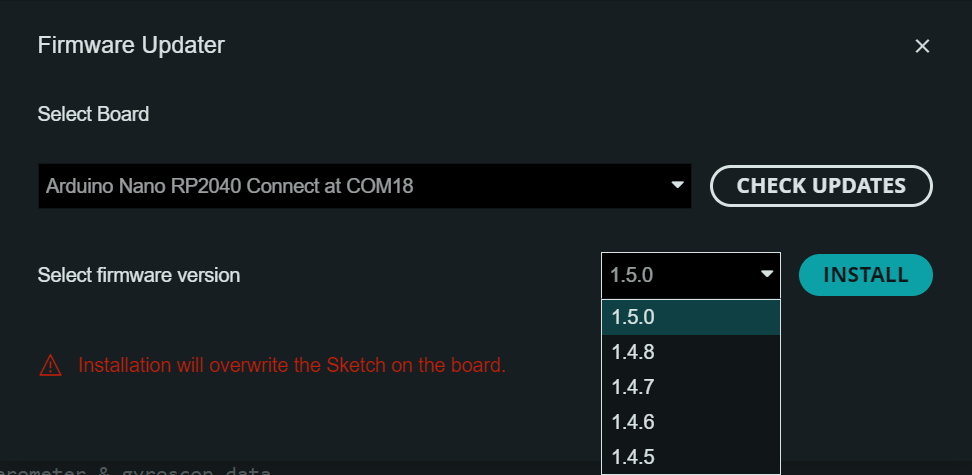
\includegraphics[width=0.8\textwidth]{exercise_micro-python/update_firmware.png}
  \caption{Update Firmware}
\end{figure}

\subsection{Using WiFi with \code{micropython}}

After this long journey (in which I unfortunately did not fight a dragon in a mountain full of gold 
and thus helped a dwarf tribe to freedom). It was possible to connect to the WiFi using the code 
shown above resulting in the following output:

\begin{figure}[H]
  \centering
  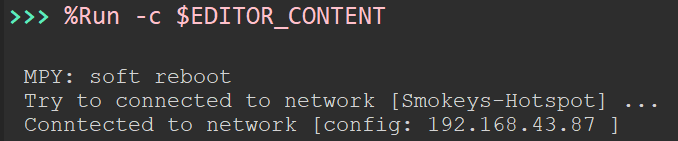
\includegraphics[width=1\textwidth]{exercise_micro-python/wifi_connected.png}
  \caption{WiFi Connected}
\end{figure}

\section{Exercise 3.3: Sending data from the Arduino to Cumulocity IoT}

The last exercise was to send data from the Arduino to Cumulocity IoT. This was done using the code 
shown in \code{main.py} of the repository which could be found \href{https://github.com/Smokey95/AIN_Ubiquitous_Computing/tree/main/exercise/sheet%202}{\textit{here}}.
Cause the code is very huge I will not post it here but it is well documented and should be self-explanatory.
\newline
\newline
For this exercise it would also be required to access the sensors on the board.
Access the boards sensors was done using the \code{LSM6DSOX} library and the code 
provided \href{https://micropython-lsm6dsox.readthedocs.io/en/latest/examples.html}{\textit{here}}.
\textbf{Note:} The \code{SDA} and \code{SCL} pins are different on the Arduino board and has to 
be changed like shown \href{https://docs.arduino.cc/tutorials/nano-rp2040-connect/rp2040-openmv-mlc}{\textit{here}}.
To import the library i wrote a small script \code{import\_lsm6dsox.py} which imports the library using \code{mip}.
\newline
\newline
After setting up everything it was possible to send data to Cumulocity IoT resulting in the following output:
\begin{figure}[H]
  \centering
  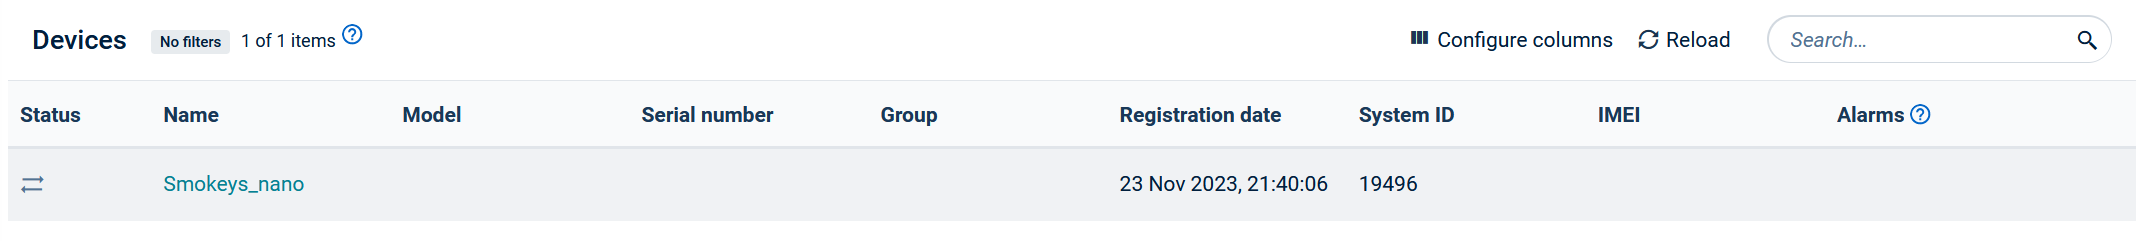
\includegraphics[width=1\textwidth]{exercise_micro-python/send_data.png}
  \caption{Send Data}
\end{figure}

\chapter{Exercise 4: Machine Learning}
\section{Exercise 4: Machine Learning}
Exercise number four is about machine learning. Therefore we will use \textit{Python} and \textit{Tensorflow} 
to analyze and work on Smarthome data captured in a \textit{.csv} file. 
As this is done in an \textit{Jupyter Notebook} the task could be done local or in \textit{Google Colab}.

\subsection{Setup}
As i prefer to work on my local machine and the \textit{Jupyter Notebook} file which was handed out 
worked with \textit{Google Colab} i had to do some changes to the code.
These sections are marked with \textit{Requirements WSL} in the \textit{Jupyter Notebook} file 
which can be found in the \textit{exercise/sheet 4} folder.

\subsection{Documentation}
As the exercises were done in the \textit{Jupyter Notebook} file, the documentation of the two exercises 
is also done there as markdown text and code comments.
Please see the \textit{Jupyter Notebook} file in the \textit{exercise/sheet 4} folder at 
\url{https://github.com/Smokey95/AIN_Ubiquitous_Computing}.

\chapter{Exercise 5: Cumulocity}
\section{Exercise 5: Cumulocity}
Exercise number five is about \textit{Cumulocity}. There are three tasks defined in the sheet about how to 
use some features of \textit{Cumulocity} portal.

\subsection{Task 1: Dashboards}
The first task is about creating a dashboard in \textit{Cumulocity} portal. Therefore it was required to 
connect the smartphone to \textit{Cumulocity} and install the \textit{Cumulocity} app on the smartphone.
After this the smartphone could be used to collect data like the battery level, the current location gyroscope 
and accelerometer data. This data was then visualized in a dashboard in the \textit{Cumulocity} portal.

On the picture bellow you can see the dashboard as well as my location during the time i was working on this
exercise.
\begin{figure}[H]
    \centering
    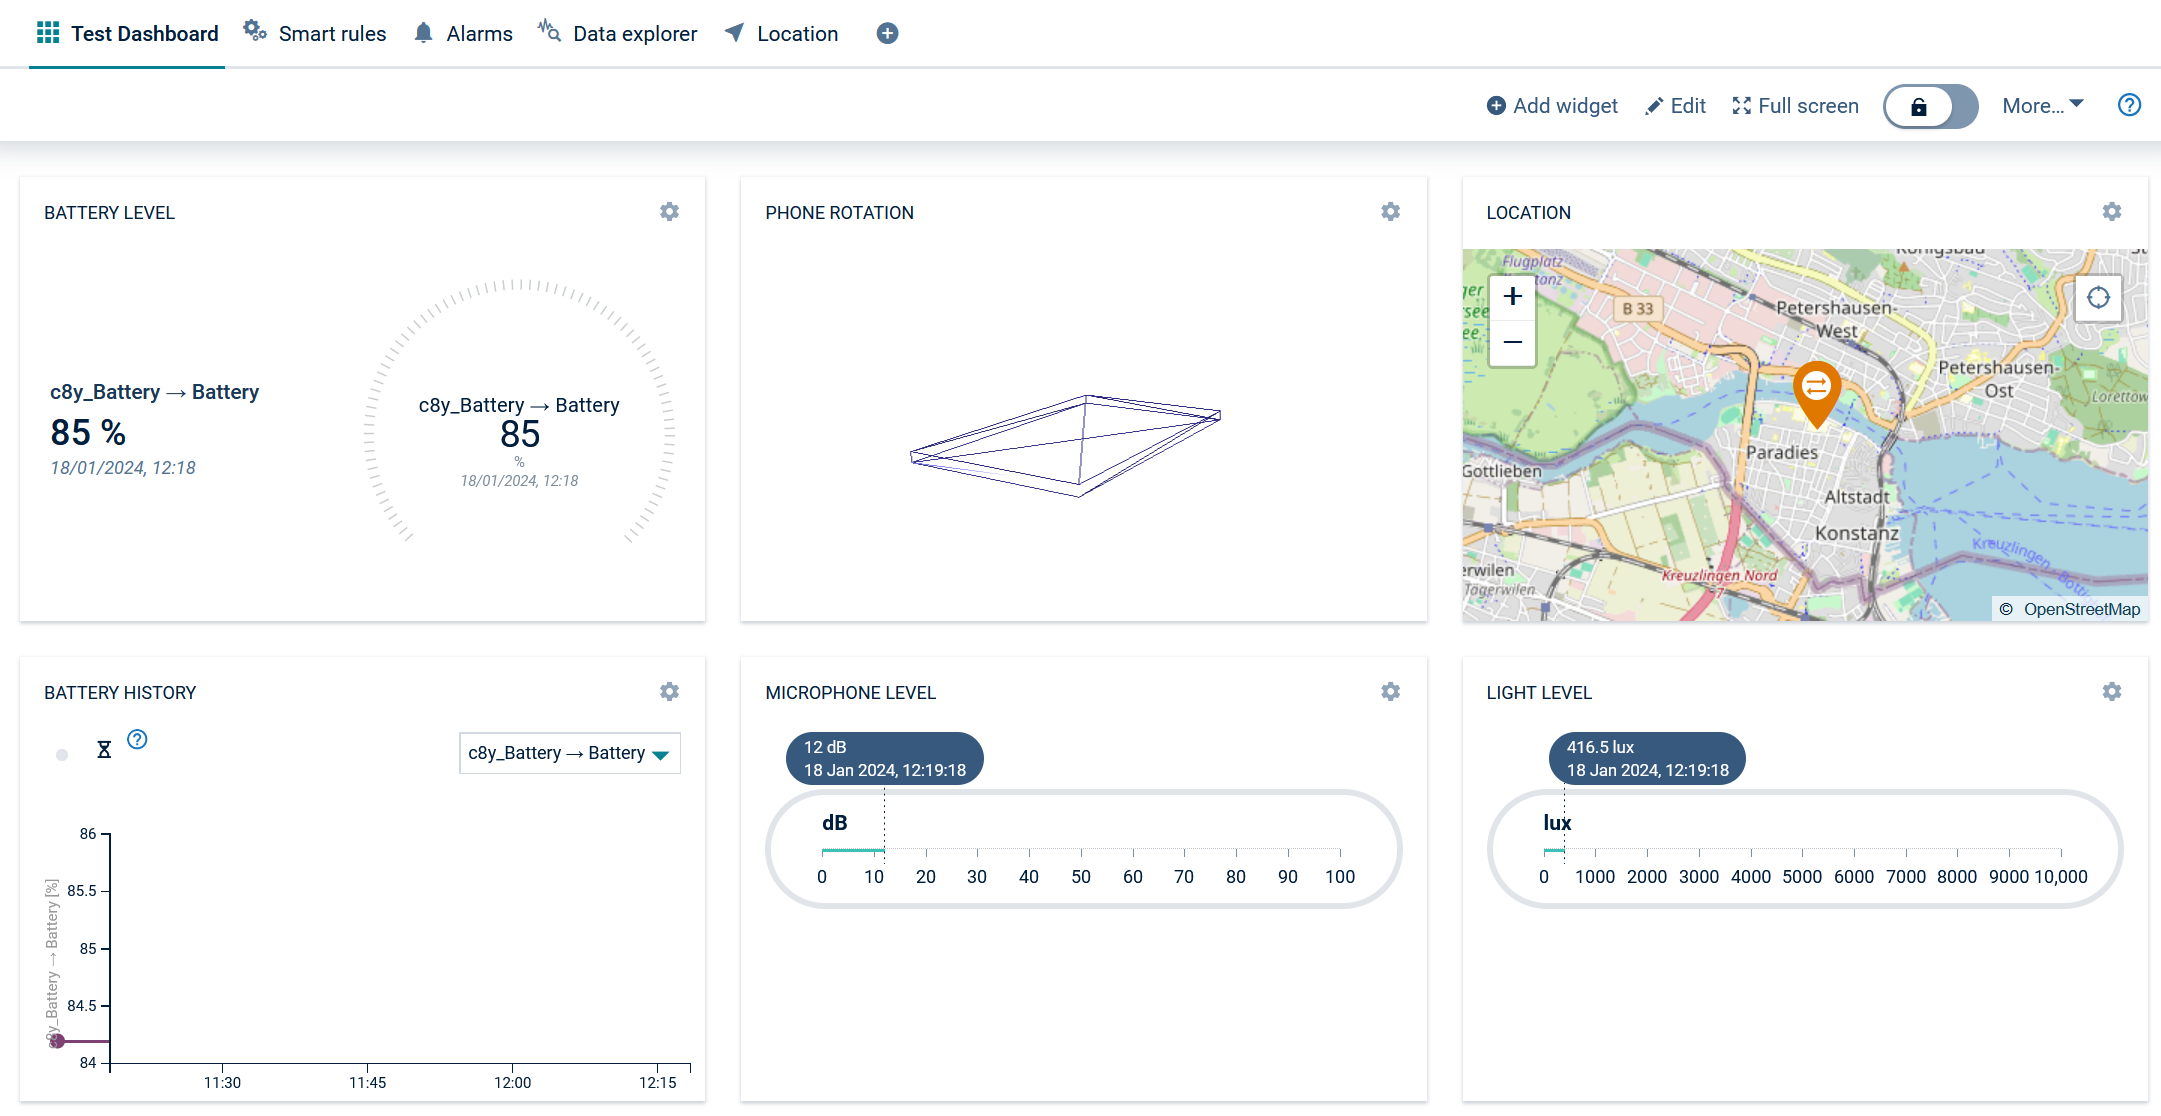
\includegraphics[width=1\textwidth]{exercise_cummolocity/task_1_dashboard.png}
    \caption{Cumulocity Dashboard}
    \label{fig:cumulocity_dashboard}
\end{figure}

\subsection{Task 2: Smart Rules}
The second task is about creating a smart rule in \textit{Cumulocity} portal. 
There we will use our already connected smartphone to trigger an alarm when it is upright or level.
Like in the first task this was straight forward following the instructions on the tutorial page.
As i did not read further at the task where the vibration alarm was set up to the next section, where it 
was described how to stop the vibration alarm again, my phone turned into a device we do not want to go 
to deep into detail here. Anyway bellow you will see the crated smart rule and the alarm which was triggered.

\begin{figure}[H]
    \centering
    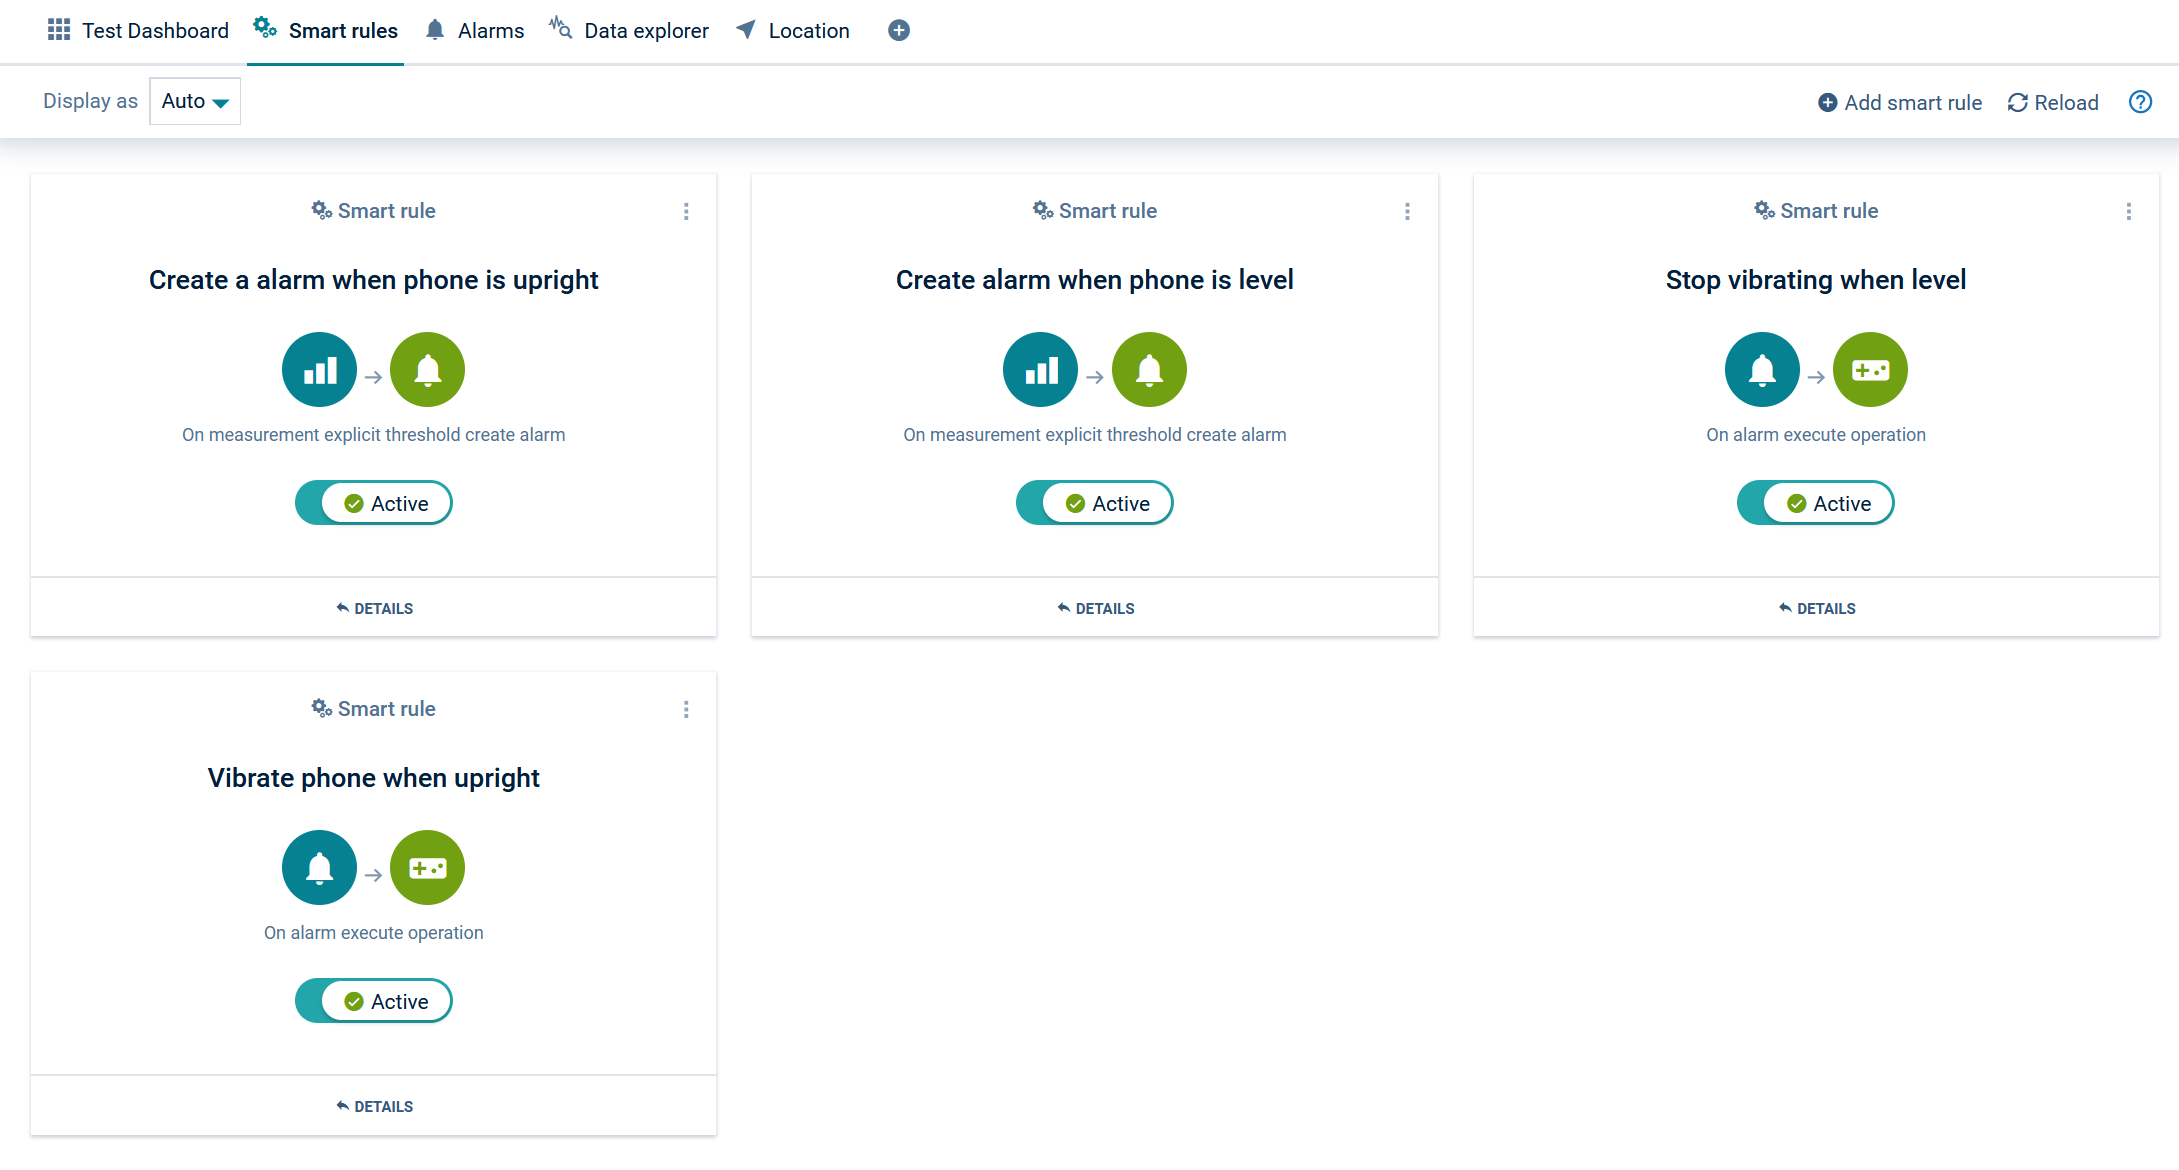
\includegraphics[width=1\textwidth]{exercise_cummolocity/task_2_smart_rules.png}
    \caption{Cumulocity Smart Rule}
    \label{fig:cumulocity_smart_rule}
\end{figure}

\begin{figure}[H]
    \centering
    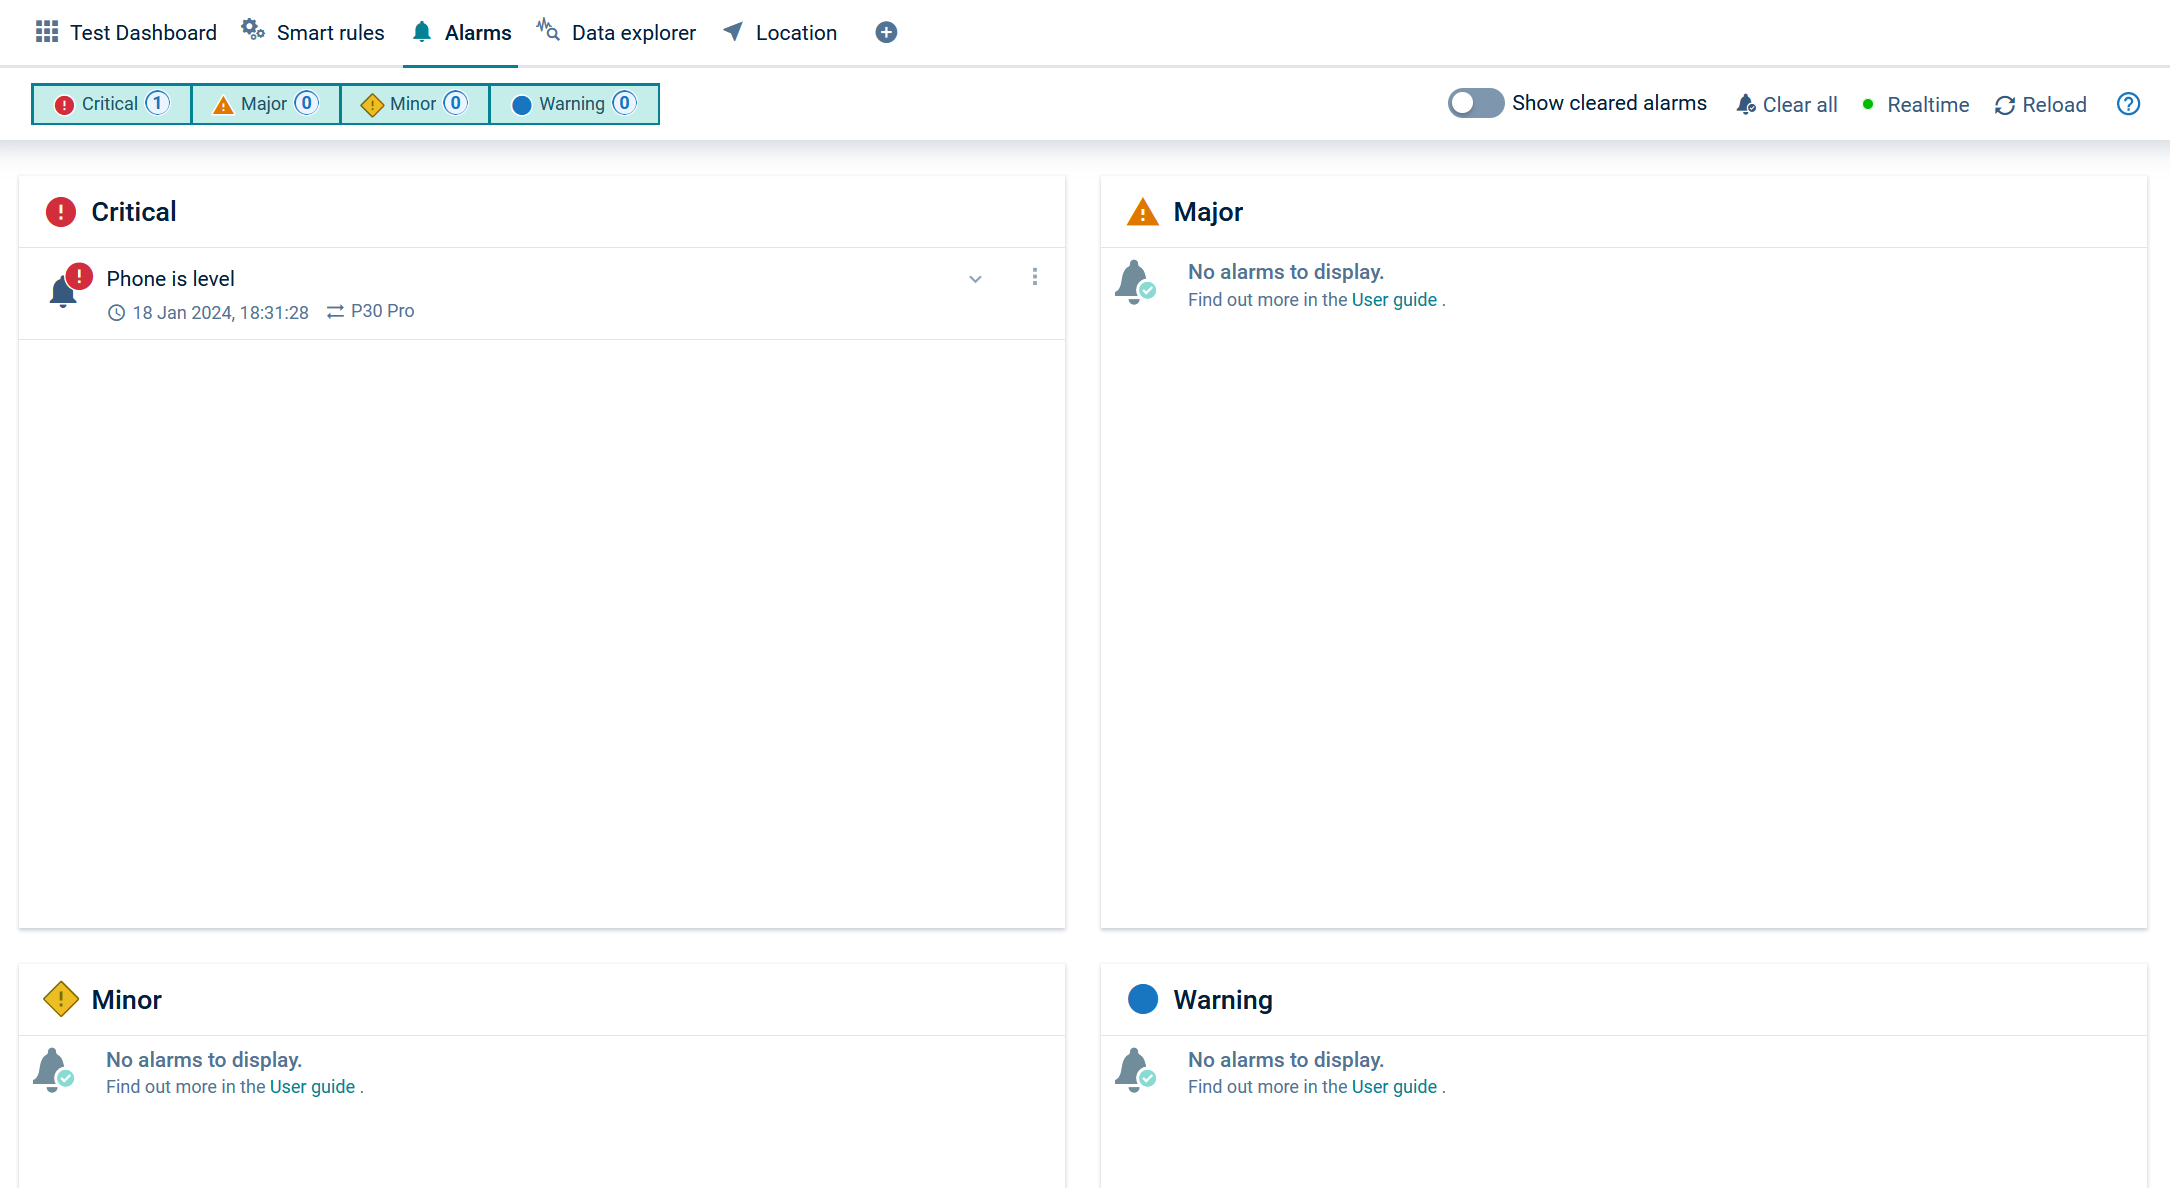
\includegraphics[width=1\textwidth]{exercise_cummolocity/task_2_alarms.png}
    \caption{Cumulocity Alarm}
    \label{fig:cumulocity_alarm}
\end{figure}

\subsection{Task 3: Analytics Builder}

The third task is about creating a analytics builder which could be seen as a more advanced version of the 
smart rules. With the analytics builder you can create more complex rules and also use the data from multiple 
devices and react on this data on a more complex way.
The task was to implement a builder which will detect if the smartphone is shaken and then trigger an alarm.
This was done by using the accelerometer data from the smartphone and a rule which will trigger an alarm if 
the acceleration is above a certain threshold. As before this was straight forward following the instructions 
on the tutorial page.

\begin{figure}[H]
    \centering
    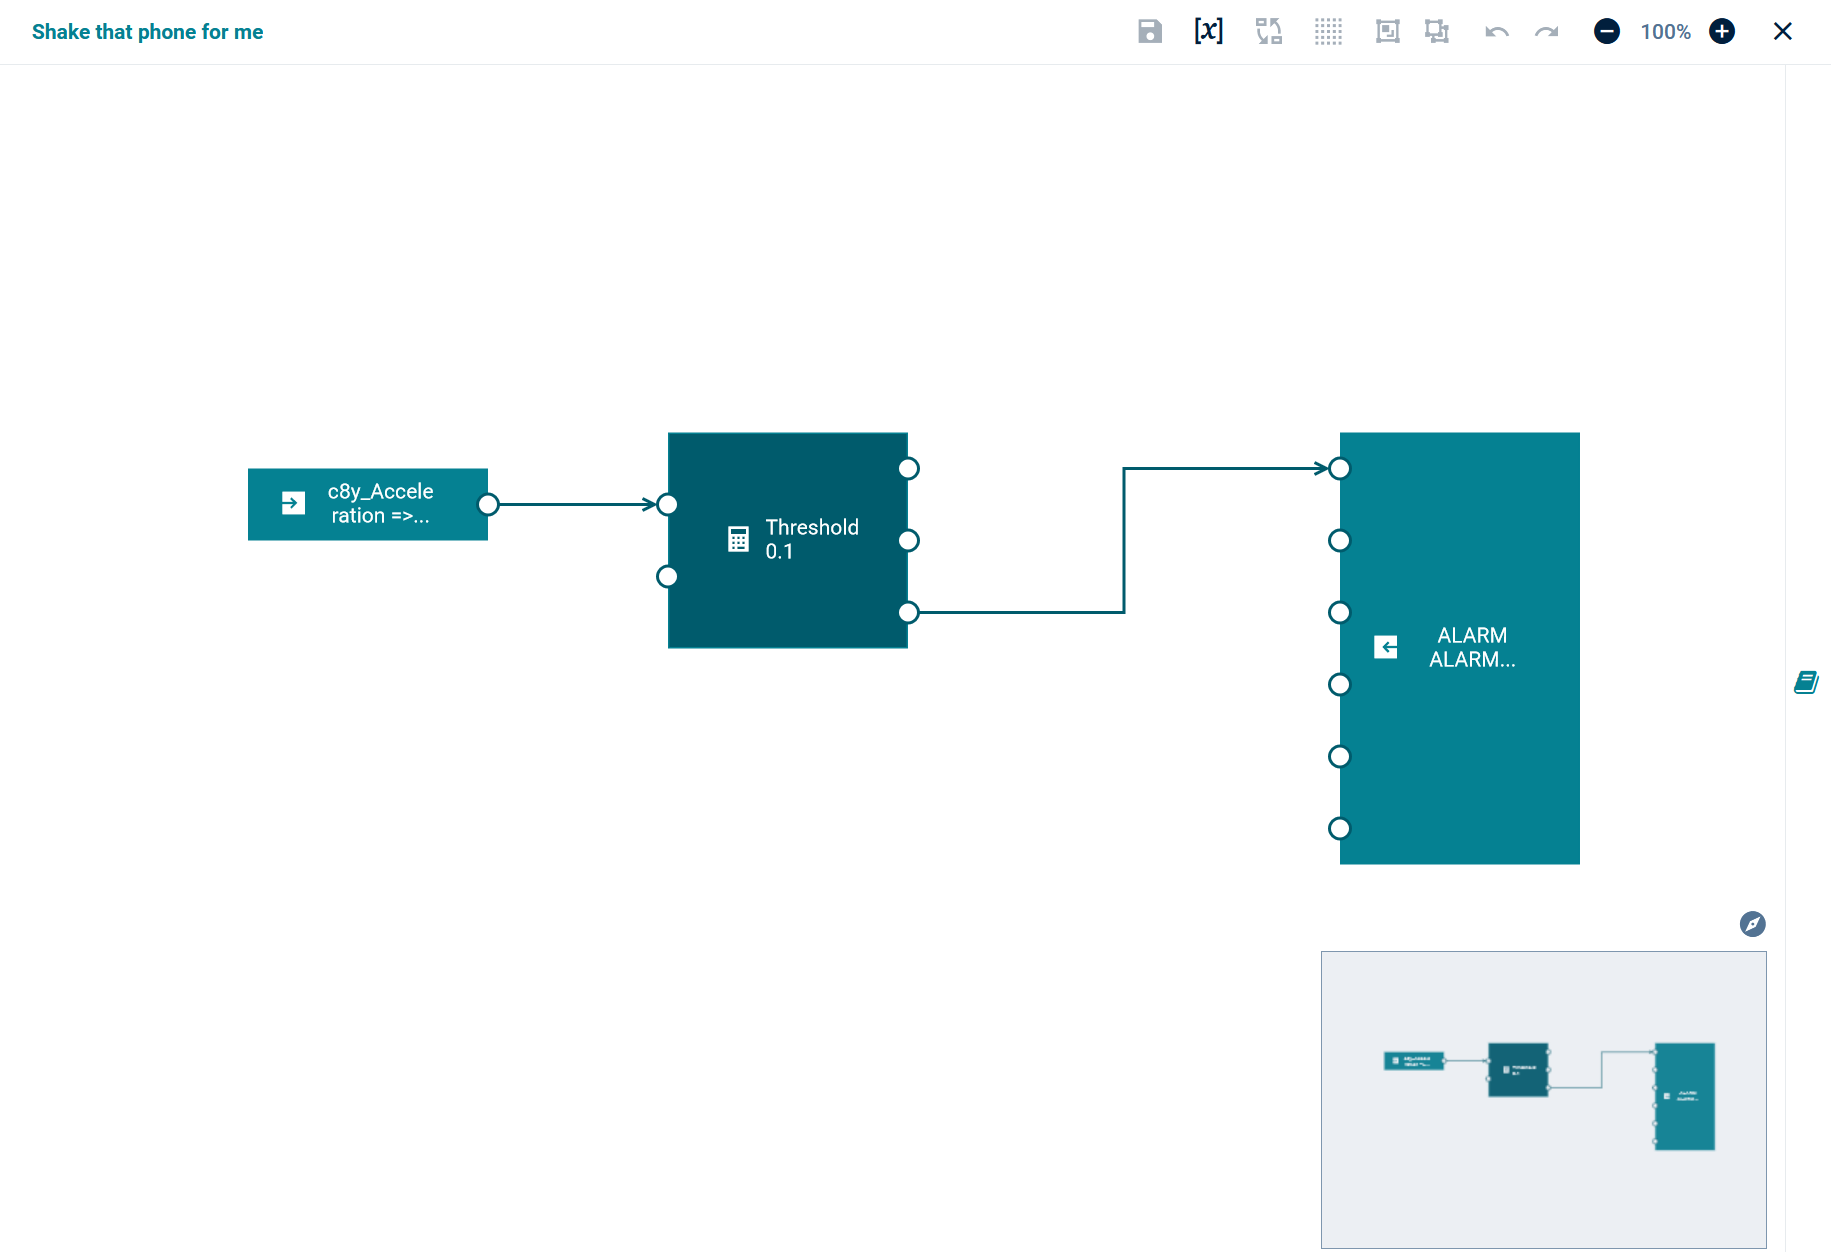
\includegraphics[width=1\textwidth]{exercise_cummolocity/task_3_analytics_builder.png}
    \caption{Cumulocity Analytics Builder}
    \label{fig:cumulocity_analytics_builder}
\end{figure}

\begin{figure}[H]
    \centering
    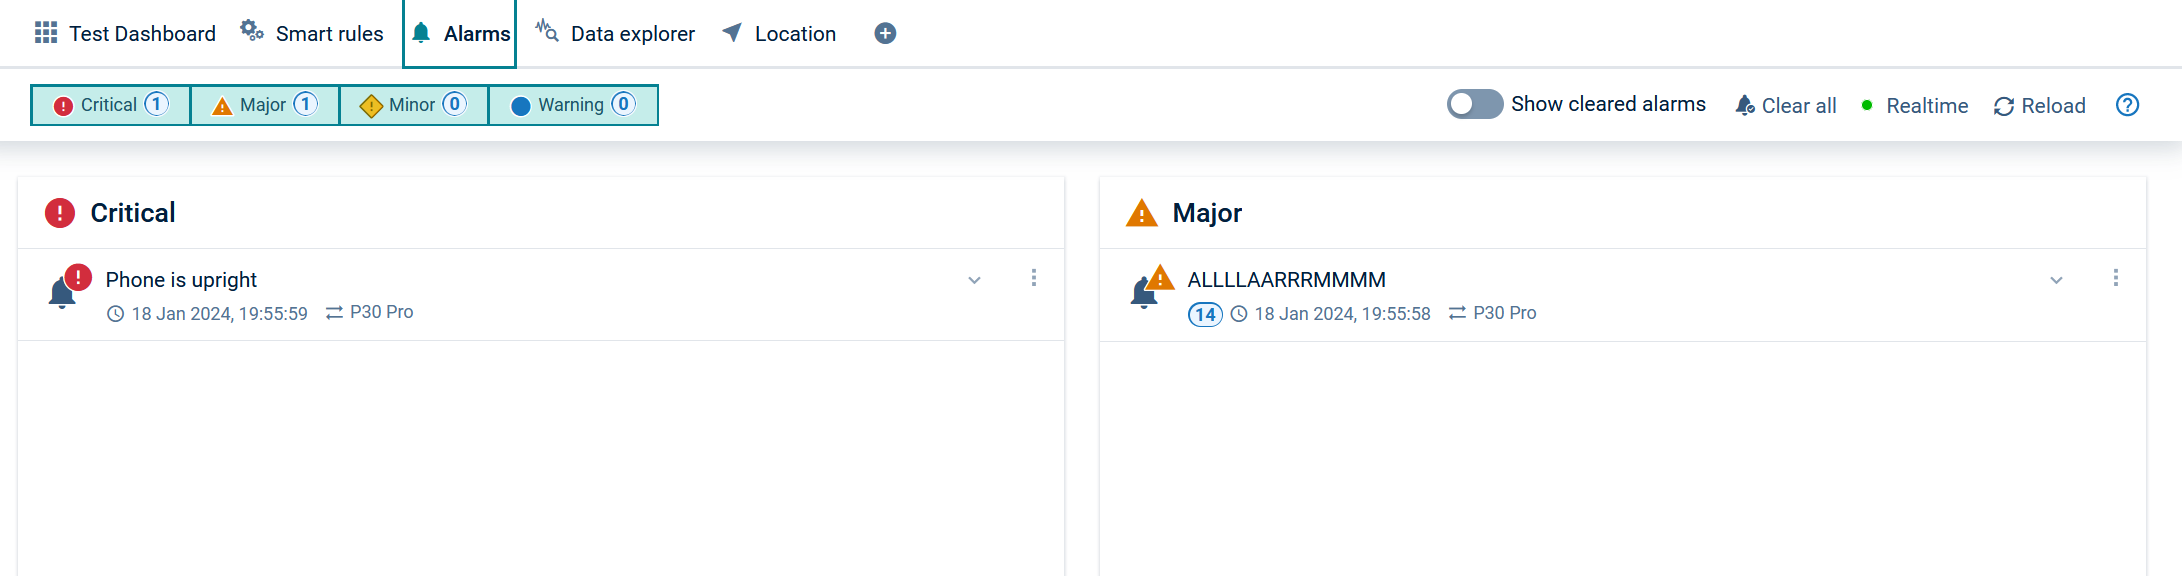
\includegraphics[width=1\textwidth]{exercise_cummolocity/task_3_alarms.png}
    \caption{Cumulocity Alarm}
    \label{fig:cumulocity_alarm}
\end{figure}

\chapter{Exercise 6: Home Assistant}
\section{Exercise 6: Home Assistant}
The last exercise is about \textit{Home Assistant}. 
There are several tasks defined in the sheet about how to setup and use some features of \textit{Home Assistant}.

\subsection{Task 1: Setup}
As \textit{Home Assistant} recommends to use a Raspberry Pi to run the \textit{Home Assistant} server 
which is in my opinion more realistic than using a local virtual machine, i decided to use a Raspberry Pi 3B+ 
to run the \textit{Home Assistant} server. Image belows shows the \textit{Home Assistant} setup after the system was 
installed like described \href{https://www.home-assistant.io/installation/raspberrypi}{\textit{here}}.

\begin{figure}[H]
    \centering
    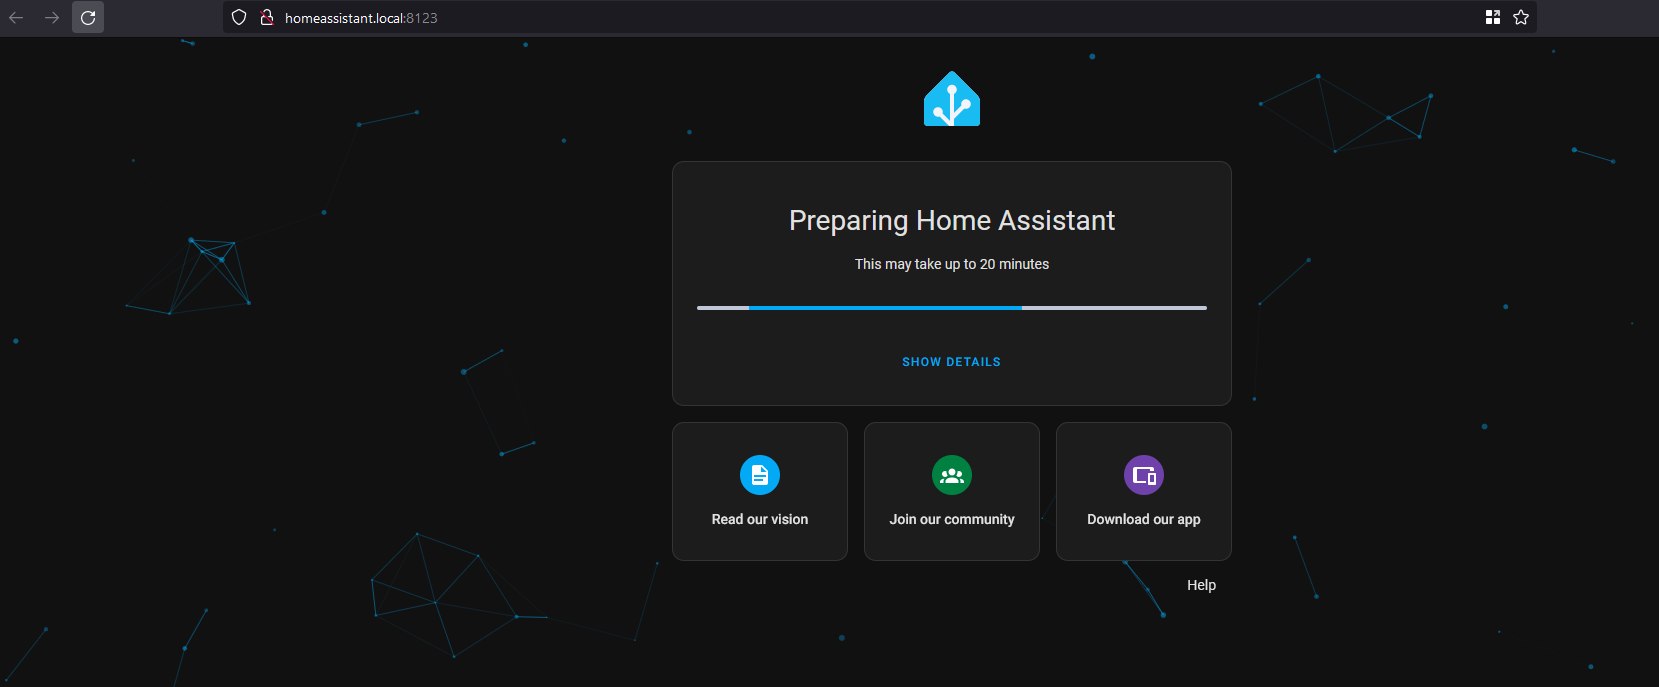
\includegraphics[width=1\textwidth]{exercise_home-assistant/setup.png}
    \caption{Home Assistant Setup}
    \label{fig:home_assistant_setup}
\end{figure}

After the setup was done the dashboard will be shown as seen in the image below.

\begin{figure}[H]
    \centering
    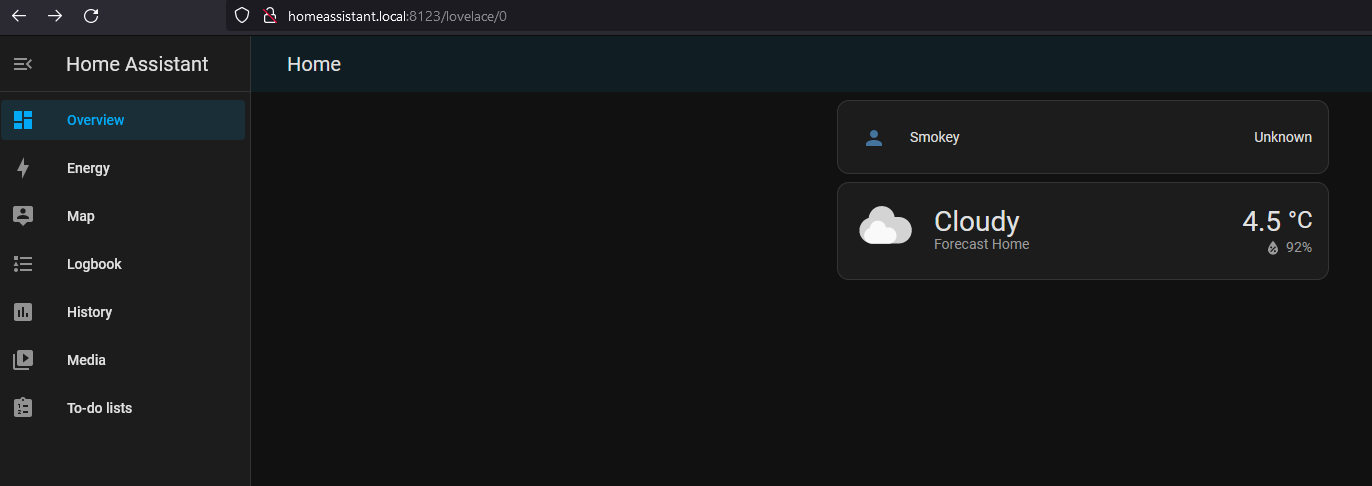
\includegraphics[width=1\textwidth]{exercise_home-assistant/dashboard_blank.png}
    \caption{Home Assistant Dashboard}
    \label{fig:home_assistant_dashboard}
\end{figure}

\subsection{Task 2: Add first service}
As first service it is required to add the \textit{AccuWeather} service to \textit{Home Assistant}.
This was mainly done like described in the tutorial \href{https://www.home-assistant.io/integrations/accuweather}{\textit{here}}.
Even if the default dashboard already contains a weather widget, i added this one to the dashboard as well.
Images below shows the successfully created \textit{AccuWeather Service} and the dashboard with the new widget.

\begin{figure}[H]
    \centering
    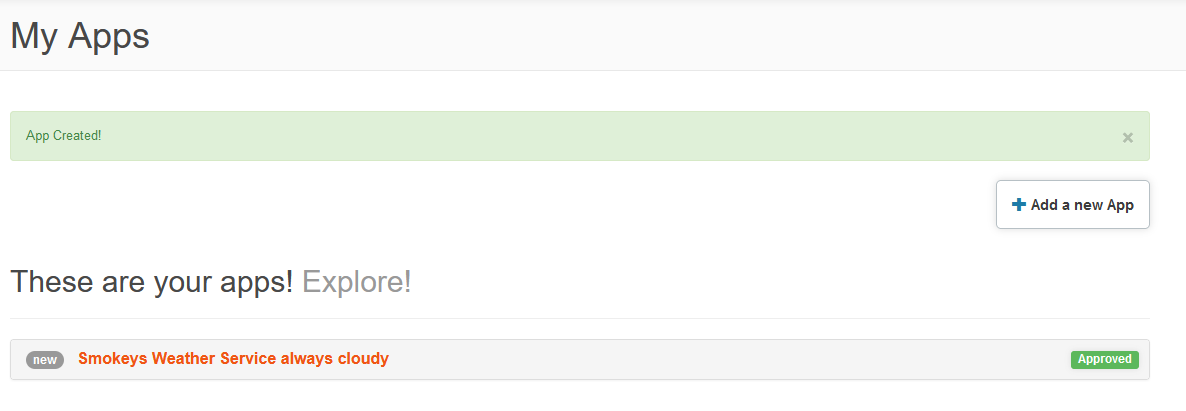
\includegraphics[width=1\textwidth]{exercise_home-assistant/accuweather.png}
    \caption{Home Assistant AccuWeather Service}
    \label{fig:home_assistant_accuweather_service}
\end{figure}

\begin{figure}[H]
    \centering
    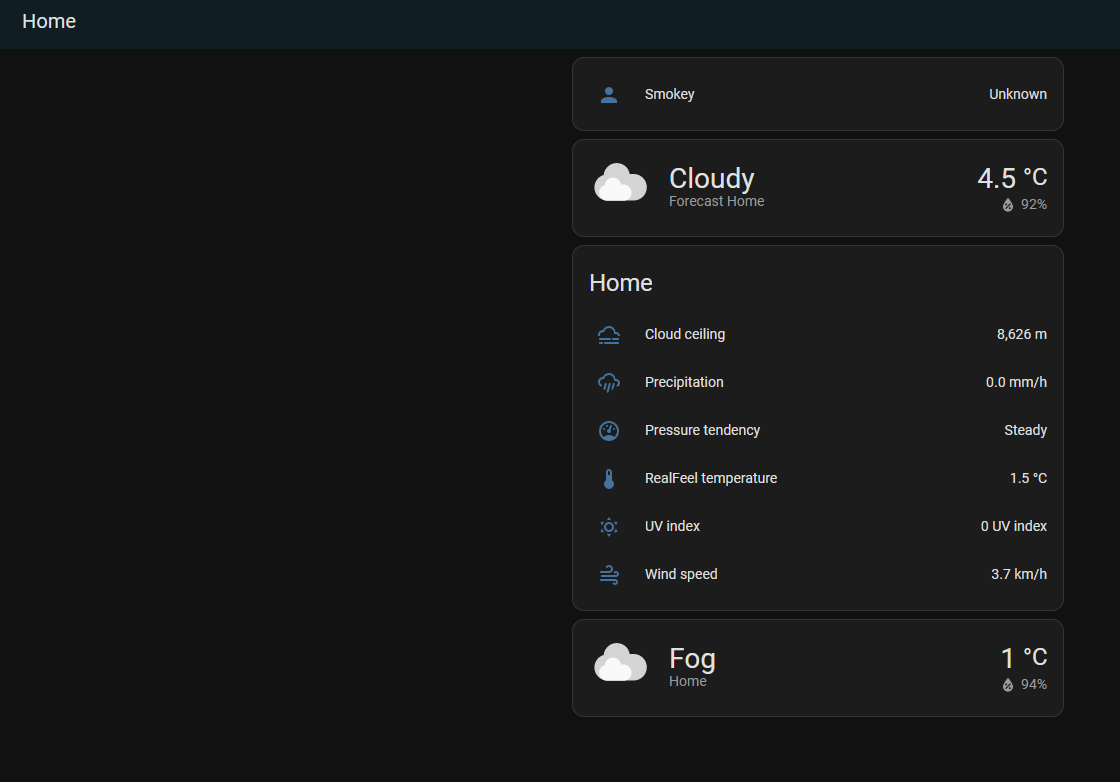
\includegraphics[width=1\textwidth]{exercise_home-assistant/dashboard_accuweather.png}
    \caption{Home Assistant Dashboard with AccuWeather Widget}
    \label{fig:home_assistant_dashboard_accuweather}
\end{figure}

\subsection{Task 3: Add first automation}
The third task is about adding the first automation to \textit{Home Assistant}.
Therefore it will be required to create a Telegram bot and add it to \textit{Home Assistant}. As i am not using 
Telegram i decided to use the \textit{Discord} bot instead. This was done like described in the tutorial 
\href{https://www.home-assistant.io/integrations/discord}{\textit{How to add discord bot}}.

After creating the new Discord application as described it will be shown in the Discord developer portal like 
shown in the image below.

\begin{figure}[H]
    \centering
    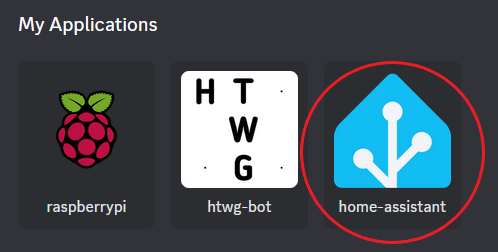
\includegraphics[width=1\textwidth]{exercise_home-assistant/discord_app.png}
    \caption{Discord Bot App View}
    \label{fig:discord_bot}
\end{figure}

After adding the Discord bot to \textit{Home Assistant} via the \textit{Devices \& services Integration} and to a 
private Discord server i used other bots before i was able to create a first automation.
Therefore the \textit{Developer Tools} were used to change the \textit{notification} service like shown in the 
image below.

\begin{figure}[H]
    \centering
    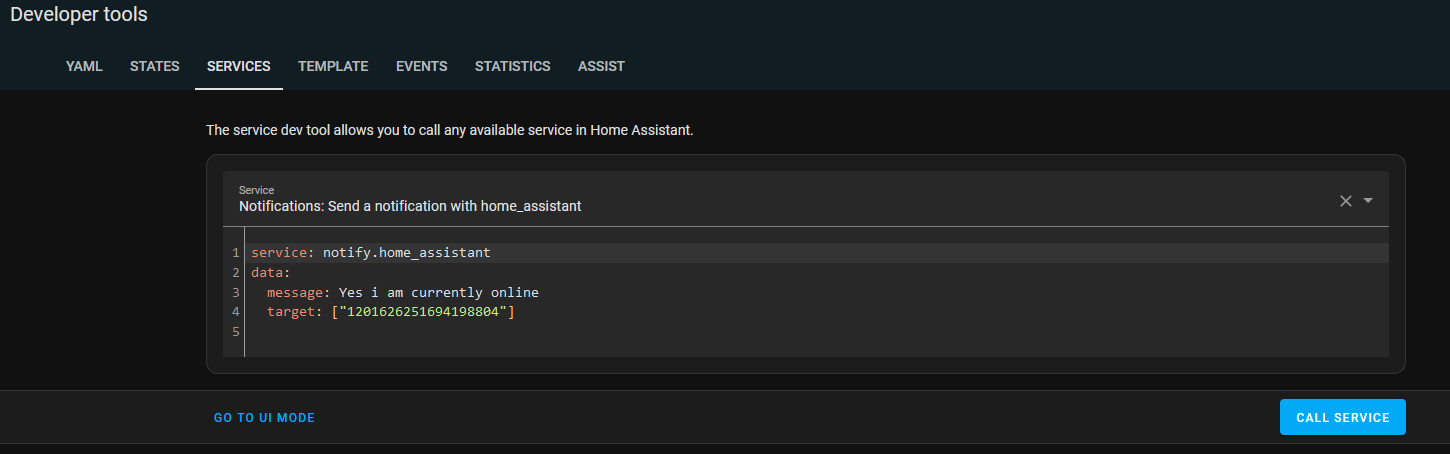
\includegraphics[width=1\textwidth]{exercise_home-assistant/service_yaml.png}
    \caption{Home Assistant Notification Service}
    \label{fig:home_assistant_notification_service}
\end{figure}

The target which is used in the \textit{target} field is the channel id of the channel where the Discord bot will 
send the messages to. Testing the service via the \textit{Call Service} button will send a message to the Discord 
channel like shown in the image below.

\begin{figure}[H]
    \centering
    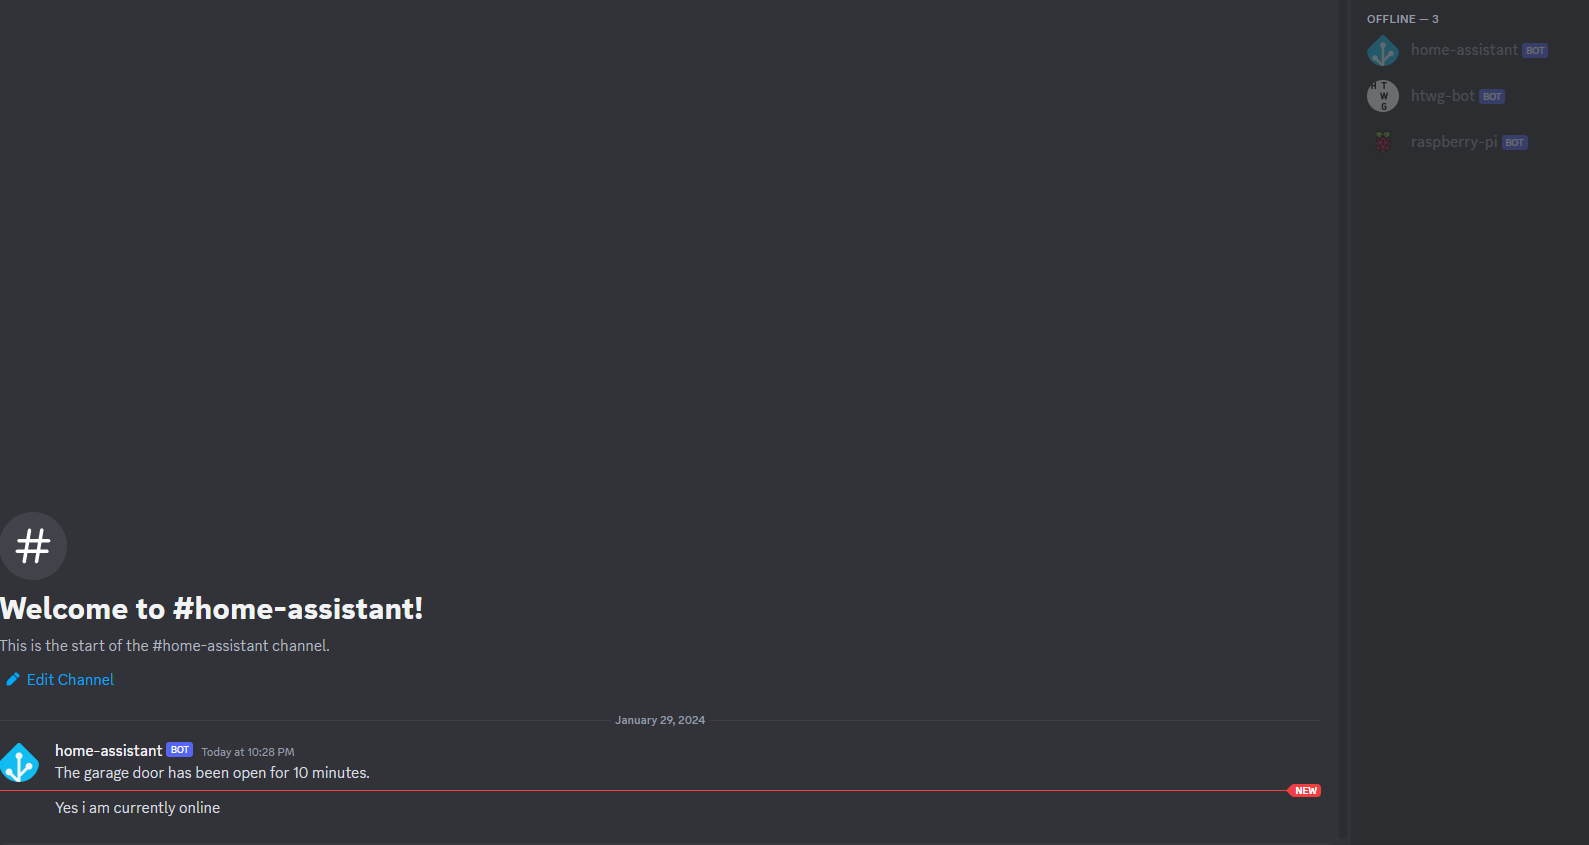
\includegraphics[width=1\textwidth]{exercise_home-assistant/bot_message.png}
    \caption{Discord Message from Home Assistant}
    \label{fig:discord_message}
\end{figure}


\subsection{Task 4: Add a periodical automation}
The fourth task is about adding a periodical automation to \textit{Home Assistant}.
Therefore the previous created notification service will be used to send a message to the Discord channel periodically.
Therefore I decided to use a message pattern like shown in the image bellow which will check the sun state and read the 
temperature data from the \textit{AccuWeather} service.
At the current version the notification will be send only once at minute 5 of every hour but can easily be extended to 
send the message every 5 minutes or every hour by adding more \textit{trigger} sections to the automation.

\begin{minted}
  [
    frame=lines,
    framesep=2mm,
    baselinestretch=1.2,
    linenos
  ]
  {C}

  trigger:
  - platform: time_pattern
    minutes: "5"
  - platform: time_pattern
    minutes: "10"
  ...
\end{minted}

The result of the automation can be seen in the image below as well as the discord notification which was send to the 
channel.

\begin{figure}[H]
    \centering
    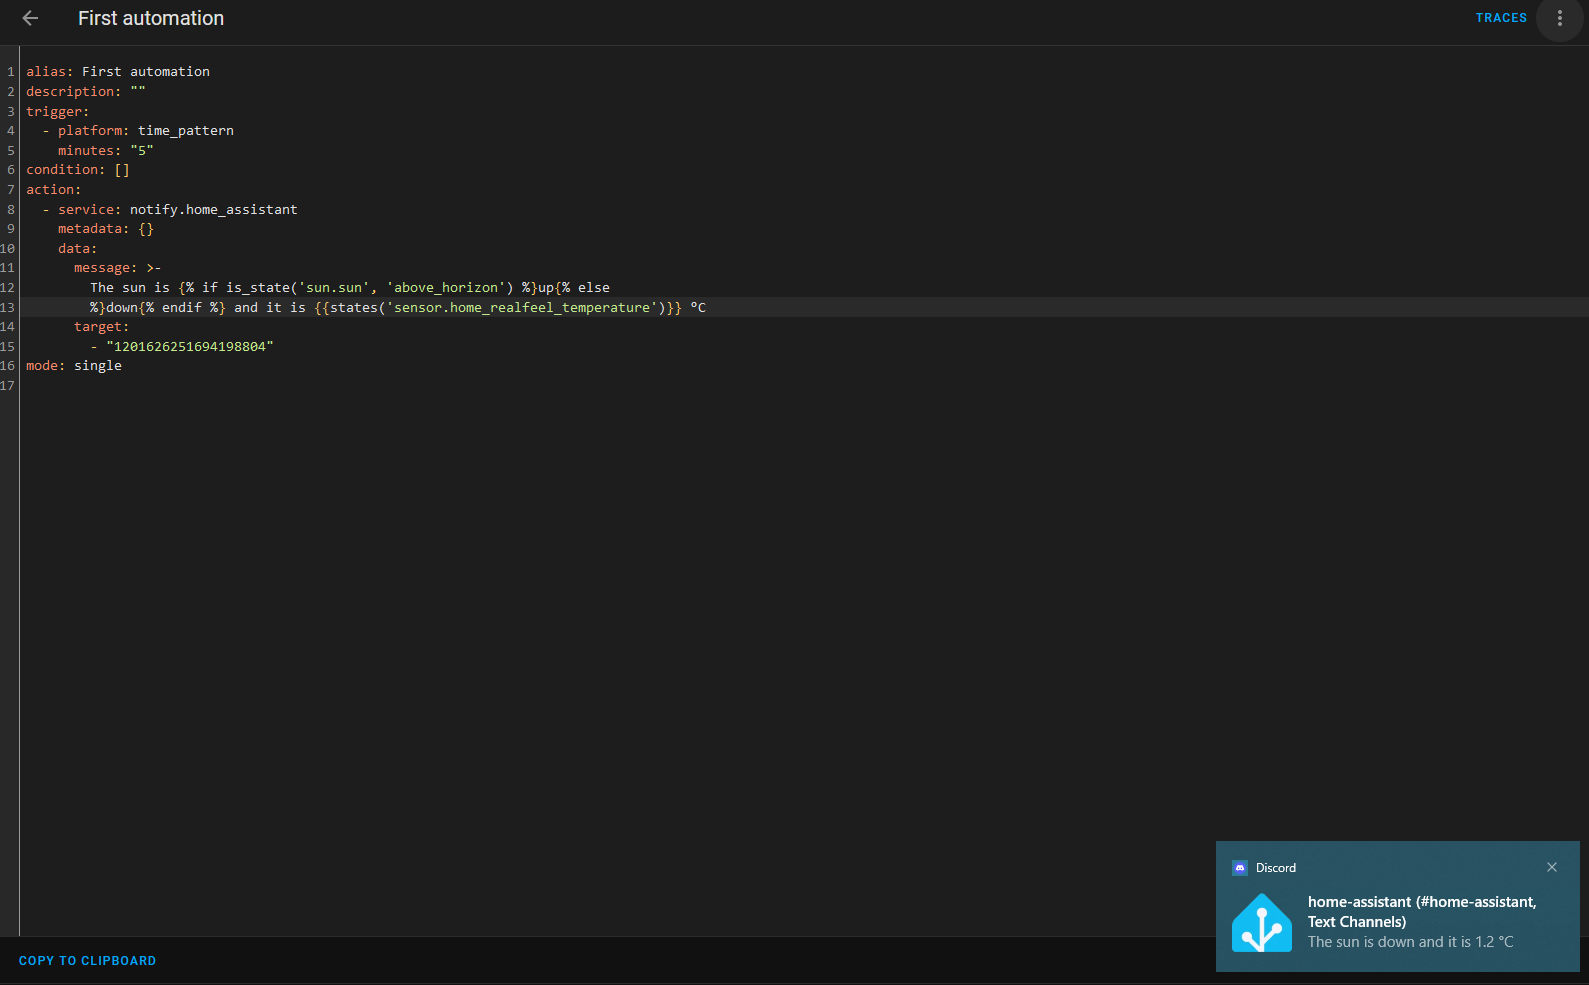
\includegraphics[width=1\textwidth]{exercise_home-assistant/automation.png}
    \caption{Discord Periodical Message from Home Assistant}
    \label{fig:discord_periodical_message}
\end{figure}

\subsection{Task 5: Smart Home Planning}
The last task is about planning a smart home system.
Therefore it was required to create floor plans for at least a basement floor as well as a ground floor and a first floor.
First i decided to create a floor plan using a online tool but most tools i found would need a little bit more time to 
get used to them. Therefore i decided to use the well known tool \textit{Paint} to create the floor plans.

\subsubsection{Import Floor Plan}
To use the floor plans in \textit{Home Assistant} it is required to import them as image files.
Therefore i created a new folder \textit{www} in the \textit{Home Assistant} configuration folder and copied the images 
into this folder. This was done using the \textit{Studio Code Server} extension which makes it possible to use the 
\textit{Visual Studio Code} editor in the browser and furthermore makes it easy to create and edit files in the 
\textit{Home Assistant} configuration folder.

After importing the images and restarting the \textit{Home Assistant} server the images can be used in the 
\textit{Home Assistant} dashboards. I would renewcommand to set the \textit{panel\_custom} configuration to 
\textit{true} to make it possible to use the images as background images for the dashboards (so they are not compressed).

\subsubsection{Device List}
To make a interactive floor plan using badges it would be required to add all devices to the \textit{Home Assistant} to 
control them. As i do not have any smart home devices i decided to just mark the devices in the floor plan like shown bellow.
As an example there is an badge added to the ground floor using the available sun sensor.

\begin{figure}[H]
    \centering
    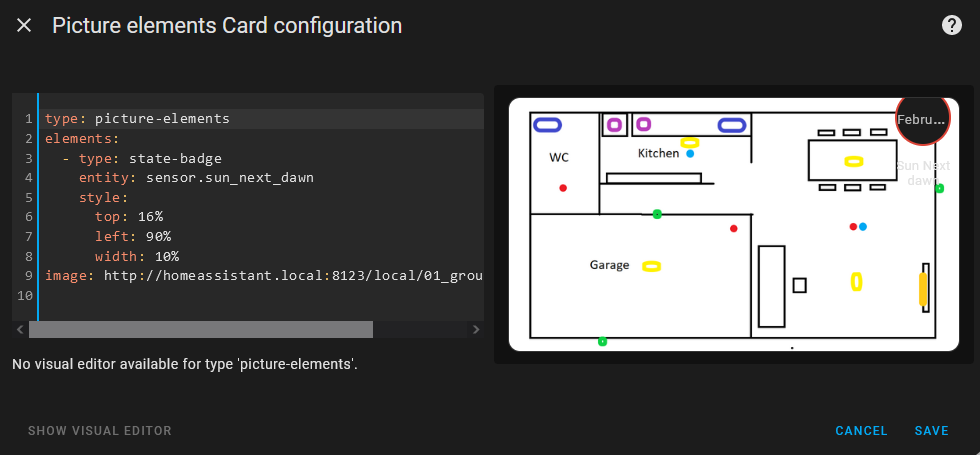
\includegraphics[width=1\textwidth]{exercise_home-assistant/example_badge.png}
    \caption{Ground Floor with Badges}
    \label{fig:ground_floor_badges}
\end{figure}

The following list shows the devices which are used in the floor plans.
As it is designed as that all devices are connected to the power grid (not using batterys),  all devices are connected via 
WiFi.

\begin{table}[!ht]
  \centering
  \begin{tabular}{|l|l|l|}
  \hline
      Color & Device & Connection \\ \hline
      Red & Smoke Detector & WiFi \\ \hline
      Green & Security Entry Devices & WiFi \\ \hline
      Blue & Smart Environment Controller & WiFi \\ \hline
      Light Blue & Smart Environment Sensor (Temperature, Humidity, CO2) & WiFi \\ \hline
      Yellow & Smart Lightning System & WiFi \\ \hline
      Orange & Smart Entertainment System & WiFi \\ \hline
      Purple & Smart Power Consumption System & WiFi \\ \hline
  \end{tabular}
\end{table}

Because of my good experience using \textit{MQTT} which was also used for my final project i would use \textit{MQTT} to 
connect all devices to the \textit{Home Assistant} server. This would make it possible to use the \textit{MQTT} broker 
to connect all devices to the \textit{Home Assistant} server and furthermore make it possible to use the \textit{MQTT} 
broker to connect the \textit{Home Assistant} server to other services like \textit{Node\-RED}.

\subsubsection{Ground Floor}
The ground floor is designed as the main living area at will be the first page of the dashboard.

\begin{figure}[H]
    \centering
    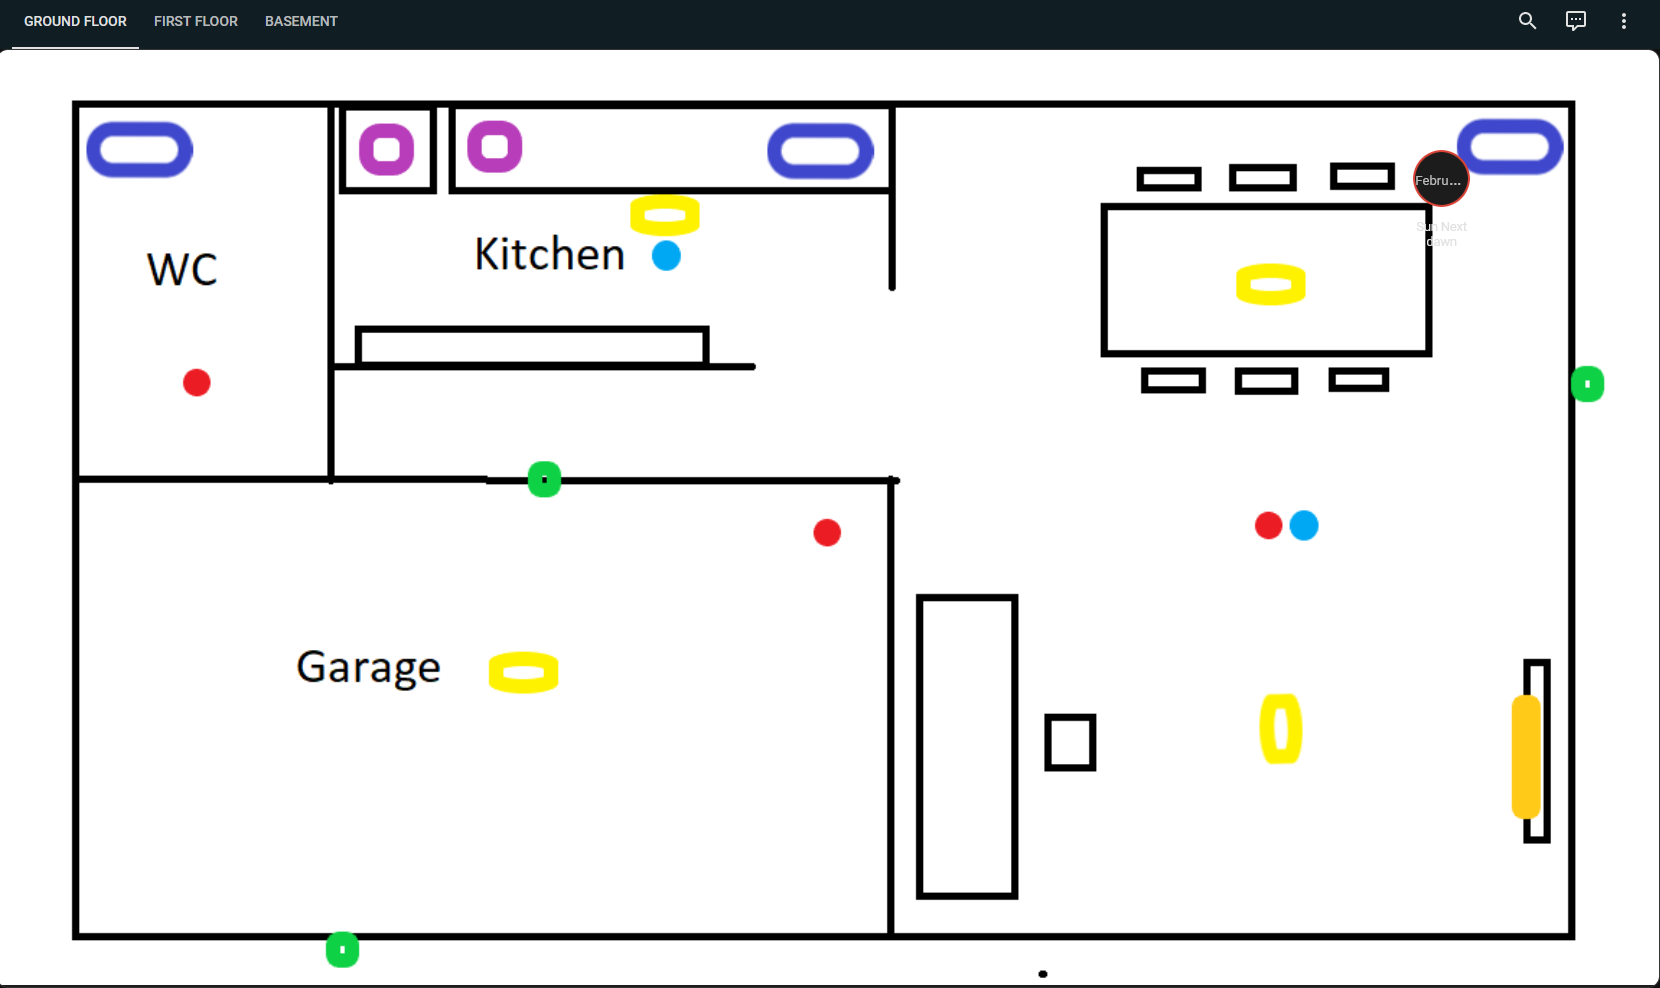
\includegraphics[width=1\textwidth]{exercise_home-assistant/plan_ground_floor.png}
    \caption{Ground Floor}
    \label{fig:ground_floor}
\end{figure}

\subsubsection{First Floor}
The first floor is designed as the sleeping area and will be the second page of the dashboard.

\begin{figure}[H]
    \centering
    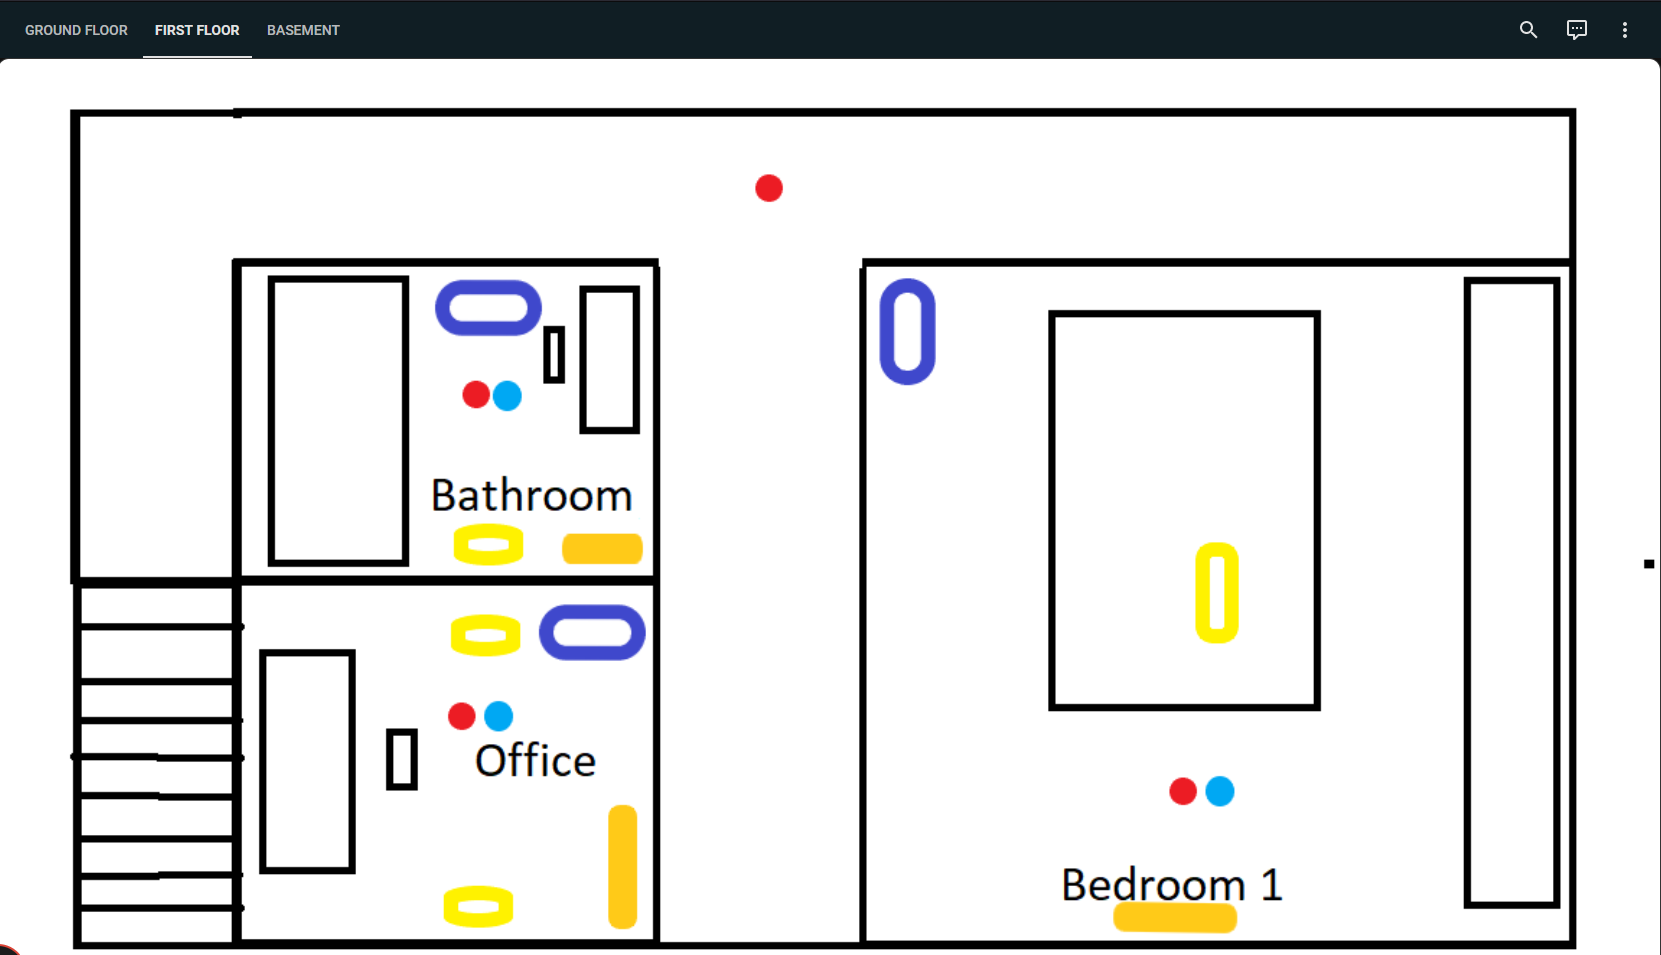
\includegraphics[width=1\textwidth]{exercise_home-assistant/plan_first_floor.png}
    \caption{First Floor}
    \label{fig:first_floor}
\end{figure}

\subsubsection{Basement Floor}
The basement floor is designed as the cleaning and workbench area and will be the third page of the dashboard.

\begin{figure}[H]
    \centering
    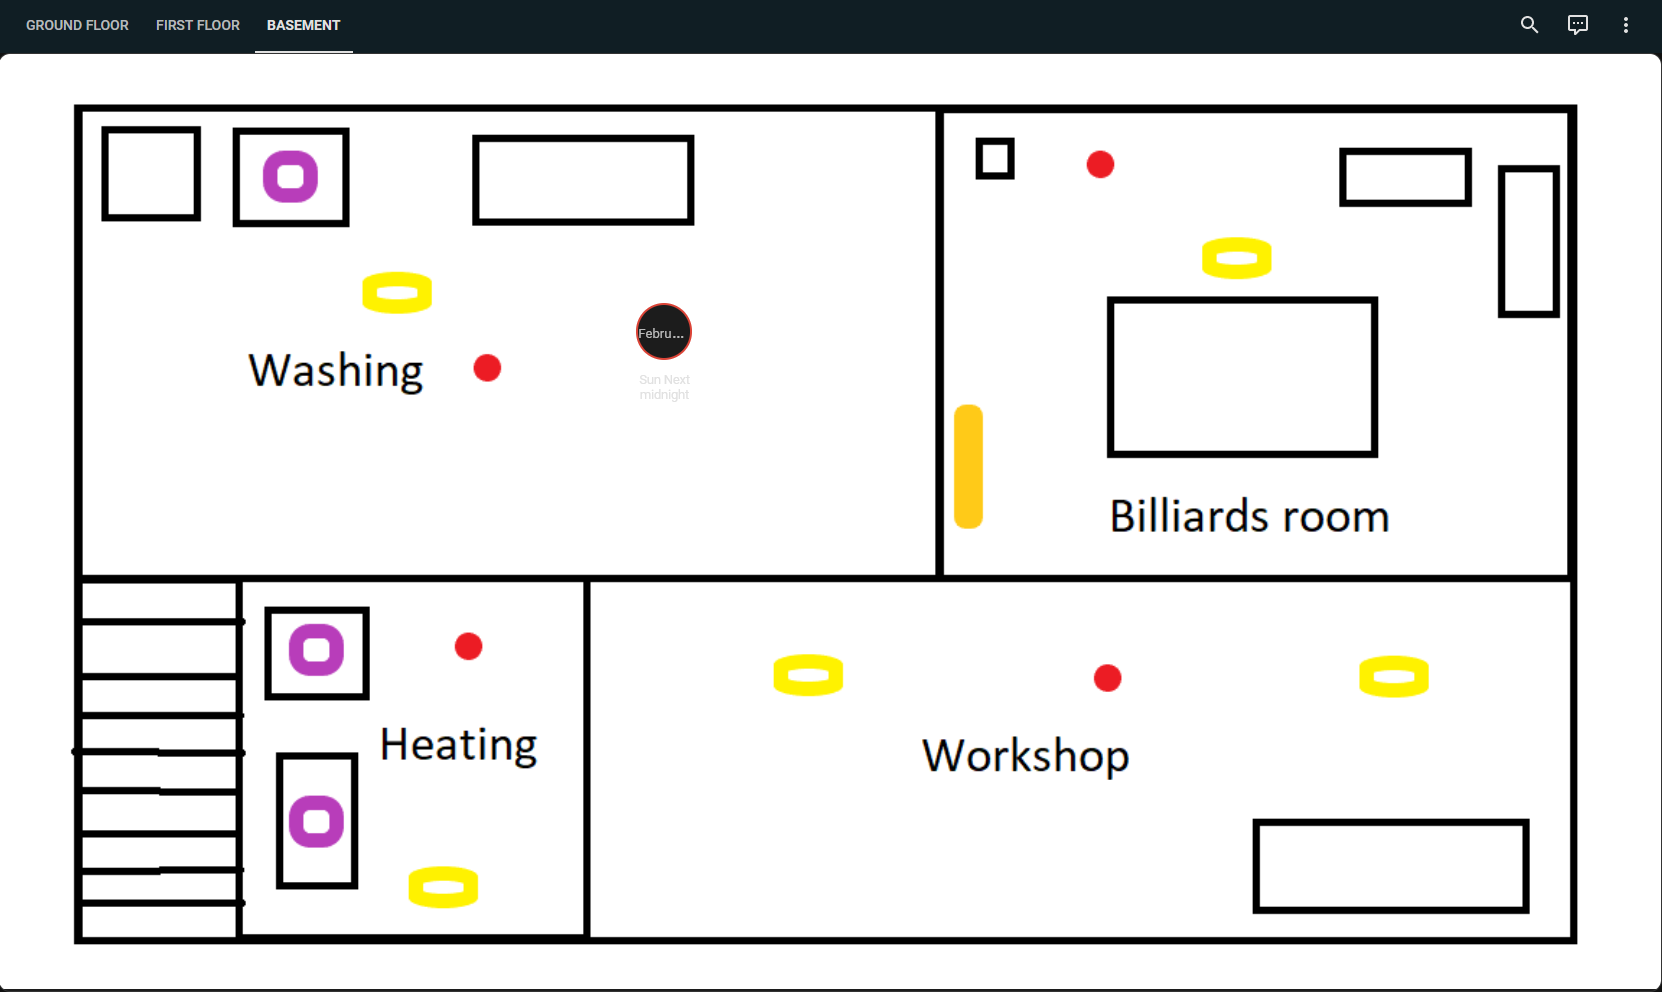
\includegraphics[width=1\textwidth]{exercise_home-assistant/plan_basement_floor.png}
    \caption{Basement Floor}
    \label{fig:basement_floor}
\end{figure}

\subsubsection{Sensors}

\paragraph{Smoke Detector}
The smoke detector is designed to detect smoke and fire and will be connected to the \textit{Home Assistant} server 
using \textit{MQTT}. It should be possible to check the status of the smoke detector using the dashboard as well as 
turning them on and off. Furthermore it should be possible to get a notification if the smoke detector detects smoke or 
fire. On one side they should notice via alarm sound as well as via notification on the dashboard and via notification 
on the previously created Discord bot.

\paragraph{Security Entry Devices}
The security entry devices are designed to detect if a door or window is opened or closed and will be connected to the 
\textit{Home Assistant} server using \textit{MQTT}. It should be possible to check the status of the security entry 
devices using the dashboard. Like already realized in the final project finger print sensors should be used to 
authenticate the user. Turn the system on and off should be possible using the dashboard as well as using a 
command send to the Discord bot.

\paragraph{Smart Environment Sense}
The smart environment sense is designed to measure the temperature, humidity and CO2 level in the room and will be 
connected to the \textit{Home Assistant} server using \textit{MQTT}. It should be possible to check the status of the 
smart environment sense using the dashboard. Furthermore it should be possible to get a notification if the CO2 level 
is to high.

\paragraph{Smart Environment Controller}
The smart environment controller is designed to control the heating, cooling and ventilation system and will be 
connected to the \textit{Home Assistant} server using \textit{MQTT} as well.
It should be possible to control the heating, cooling and ventilation system using the dashboard for 
example to set the temperature or turn the system on and off.

\paragraph{Smart Lightning System}
The smart lightning system is designed to control the lights in the rooms.
It should be possible to control the lights using the dashboard for example to turn the lights on and off or to change 
the brightness of the lights. As already mentioned in the final project presentation this should only be "IoT as a 
feature" meaning that it should be possible to control the lights using the dashboard but it should also be possible to 
control the lights using physical switches.

\paragraph{Smart Entertainment System}
The smart entertainment system is designed to control the entertainment system in the rooms like the TV or the HiFi.
It should be possible to control the entertainment system using the dashboard for example to play music or to turn the 
TV on and off.

\paragraph{Smart Power Consumption System}
The smart power consumption system is designed to measure the power consumption of some devices like the Heating, 
Cooling or Kitchen devices. It should be possible to check the power consumption of the devices using the dashboard 
but also to export the data to a file to analyze the data like done in exercise 4.

%%------------------------------------------------------------------------------ References
%Adding references to table of content
\phantomsection 
\addcontentsline{toc}{chapter}{References} 

%Change bibliography name
\renewcommand{\bibname}{References}

%Print bibliography
\printbibliography

\end{document}
%%---------------------------------------------------------------------------------------------------------------------- Document End